%%%%%%%%%%%%%%%%%%%%%%%%%%%%%%%%%%%%%%%%%%%%%%%%%%%%%%%%%%%%%%%%%%%%
%PLANTILLA DE INFORMES V 1.1
%
% REQUISITO: IMPORTE EL LOGO DE LA USM CON EL NOMBRE "logousm.png"
% IMPORTE IMAGENES DE MODULOS, EXTRAER DEL WORD
%
% Material de referencia de proposito general:
% https://users.dcc.uchile.cl/~jbarrios/latex/
% http://mate.dm.uba.ar/~pdenapo/tutorial-latex/node2.html
% http://tiburondealambre.blogspot.cl/2012/01/referencias-imagenes-y-tablas-en-latex.html
% BIBLIOGRAFIA: http://logistica.fime.uanl.mx/miguel/docs/BibTeX.pdf
%
% Tratar ecuaciones en latex(muy util):
% https://ondiz.github.io/cursoLatex/Contenido/05.Ecuaciones.html
%
% detector de cosas dibujadas latex: http://detexify.kirelabs.org/classify.html
%
%%%%%%%%%%%%%%%%%%%%%%%%%%%%%%%%%%%%%%%%%%%%%%%%%%%%%%%%%%%%%%%%%%%%%%%

%----------------------PAQUETES---------------------------%
% No es necesario tocar nada de esto

\documentclass[12pt,a4paper]{article} % tipo de documento, formato

\usepackage[utf8]{inputenc}    % con tildes
\usepackage[spanish]{babel}    % arreglar problemas

\usepackage[framed,numbered,final]{mcode} %%MATLAB
\usepackage{listings}   % Permite incorporar código con d


\usepackage{graphicx} % paquete de tratado de imagenes/figuras
\usepackage{tipa} % para <
\usepackage{amssymb} % para >=

% paquete extra para ocupar [H] (obliga a que la imagen con graphicx
% se quede donde se realizó el llamado)
\usepackage{float}

% CARGAMOS 3 PAQUETES
% (AMS Math), que mejora el comportamiento y el aspecto de las ecuaciones. 
% Nos permite, por ejemplo, añadir un asterisco en el entorno equation para crear
% ecuaciones sin numerar.
%(AMS Theorem), que define los entornos teorema y demostración.
%(AMS Symbol), que carga a su vez amsfonts e incluye una colección 
%de símbolos matemáticos.
\usepackage{amsmath, amsthm, amssymb} 

\usepackage{enumerate} %permite enumerar de varias formas

\usepackage{multirow, array} % para las tablas

% construccion de un nuevo comando
\usepackage{lipsum}% http://ctan.org/pkg/lipsum
\usepackage{xcolor}% http://ctan.org/pkg/xcolor
\usepackage{xparse}% http://ctan.org/pkg/xparse
\NewDocumentCommand{\myrule}{O{1pt} O{2pt} O{black}}{%
  \par\nobreak % don't break a page here
  \kern\the\prevdepth % don't take into account the depth of the preceding line
  \kern#2 % space before the rule
  {\color{#3}\hrule height #1 width\hsize} % the rule
  \kern#2 % space after the rule
  \nointerlineskip % no additional space after the rule
}

%acomoda margenes y tipografia para que quede mas bonito
\usepackage{geometry}
\geometry{
	paper=a4paper, % Change to letterpaper for US letter
	inner=3cm, % Inner margin
	outer=3cm, % Outer margin
	bindingoffset=.5cm, % Binding offset
	top=2cm, % Top margin
	bottom=2cm, % Bottom margin
	%showframe, % Uncomment to show how the type block is set on the page
}


%---------PORTADA, TABLA DE CONTENIOS Y FIGURAS--------------%
%Esto será la portada. Solo hay que cambiar los textos
\begin{document}

\begin{titlepage}
\begin{center}
\textbf{\LARGE Universidad Técnica Federico Santa}\\[0.25cm]
\textbf{\LARGE María}\\[0.5cm]
\textbf{\large DEPARTAMENTO DE INGENIERÍA ELECTRONICA}\\[0.2cm]
\vspace{20pt}

\includegraphics{logousm.png}\\[1cm]

\par
\vspace{15pt}
\textbf{\Large ELO 314 - Laboratorio de procesamiento Digital de Señales}\\
\vspace{15pt}
\myrule[1pt][7pt]
\textbf{\LARGE Análisis y compresión de voz en MatLab}\\[0.25cm]
\vspace{15pt}
\textbf{\large  }\\
\myrule[1pt][7pt]
\vspace{55pt}
\textbf{\large Estudiante \hspace{75pt} ROL}\\
    \hspace{0pt}Rodrigo Graves\hspace{80pt} 201621009-1 \\
     Ricardo Mardones      \hspace{60pt} 201621036-9 \\
   


\vspace{30pt}
\textbf{\large Paralelo: \hspace{30pt} 1}\\

\vspace{35pt}
\textbf {\large Profesor}\\[0.2cm]
\Large { Gonzalo Carrasco}\\[0.1cm]
\textbf {\large Ayudante}\\[0.2cm]
\Large {Jaime Guzmán}\\[0.1cm]
\end{center}

\par
\vfill
\begin{center}
\textbf{Fecha : \today}\\
\end{center}

\end{titlepage}


%-------------Lista de figuras y tablas----------%
\tableofcontents % Hace el índice de contenidos. Latex organiza todo solito
\clearpage

\listoffigures %lista de figuras
\clearpage

\listoftables
\clearpage






%I
\section{Predicción lineal y síntesis de vocales}

\subsection{Generación de Tren de Impulsos}
Se crea la función $X = exciteV (N, N p)$ que representa el sonido de las cuerdas vocales mediante un tren
de impulsos, donde N es el largo de la señal en muestras y $Np$ el período en muestras. El código de la función generada se muestra a continuación:
\begin{lstlisting}[language = octave]
function y = exciteV(N,Np)
    y = zeros(1,N)
    for i = 1:N
        if mod(i-1,Np) == 0
            y(i) = 1;
    end
end
\end{lstlisting}

Posteriormente se genera un tren de impulsos de 100 Hz de duración $1~s$ muestreada a $8~kHz$, para luego escucharla y graficar su espectro en frecuencia. Lo anterior usando el script \texttt{p1\_1.m}, adjunto a la entrega.

La sección de código donde se genera la señal de tren de impulsos corresponde a:
\begin{lstlisting}[language = octave]
fs = 8000;
t =1;
f = 100;
T = fs/f;
y = exciteV(t*fs,T);
Y =   fft(y);
Ymod = abs(Y);
Ydb = 20*log10( 0.000000001 + Ymod(1:fs/2));  
plot([0:fs/2-1],  Ydb(1:fs/2));

\end{lstlisting}



El espectro obtenido para la señal generada se muestra en  la figura \ref{frec_tren}

\begin{figure}[H]
    \centering
    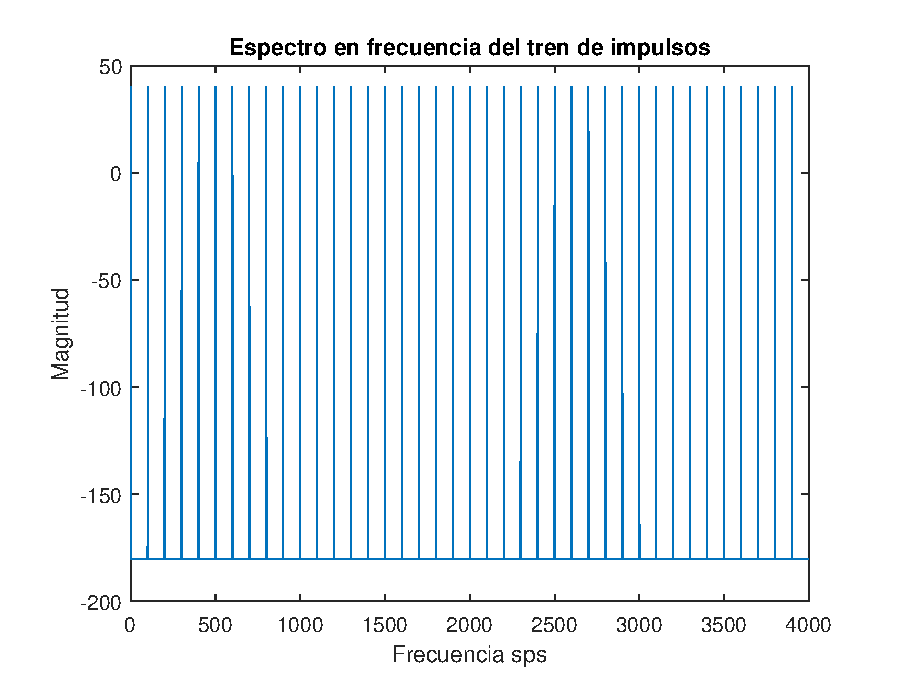
\includegraphics[scale = 0.7]{figures/p1_1frec_tren.eps}
    \caption{Espectro del tren de impulsos generada con la función \textit{exciteV}}
    \label{frec_tren}
\end{figure}

\subsection{Diseño de filtros AR óptimos usando $y = lpc(x,p)$}

Para esta parte se utilizó el código \texttt{p1\_2.m}, adjunto a la entrega.

La sección de código donde se diseñan los filtros que simulan el comportamiento del tracto vocal para cada vocal se muestra a continuación:
\begin{lstlisting}[language = octave]
load vowels

% Diseno de filtros
a_vowel_a = lpc(vowel_a,P);
a_vowel_e = lpc(vowel_e,P);
a_vowel_i = lpc(vowel_i,P);
a_vowel_o = lpc(vowel_o,P);
a_vowel_u = lpc(vowel_u,P);
\end{lstlisting}
donde $P = 15$, el cual corresponde al orden del filtro que se desea generar.

Las respuestas en frecuencia de cada vocal se muestran en las figuras \ref{fig:p1_2a} - \ref{fig:p1_2u}, donde además se destaca el primer y segundo formante.

\begin{figure}[H]
    \centering
    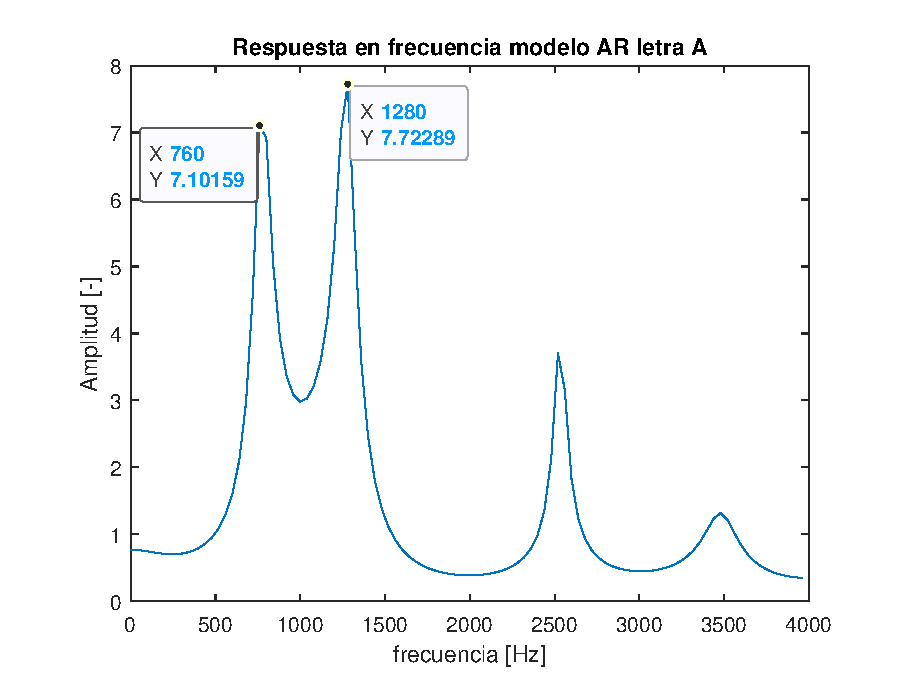
\includegraphics[width = .8\linewidth]{figures/p1_2a.eps}
    \caption{Respuesta en frecuencia de filtro estimado para simular tracto vocal haciendo letra a. Se destaca el primer y segundo formante encontrado.}
    \label{fig:p1_2a}
\end{figure}

\begin{figure}[H]
    \centering
    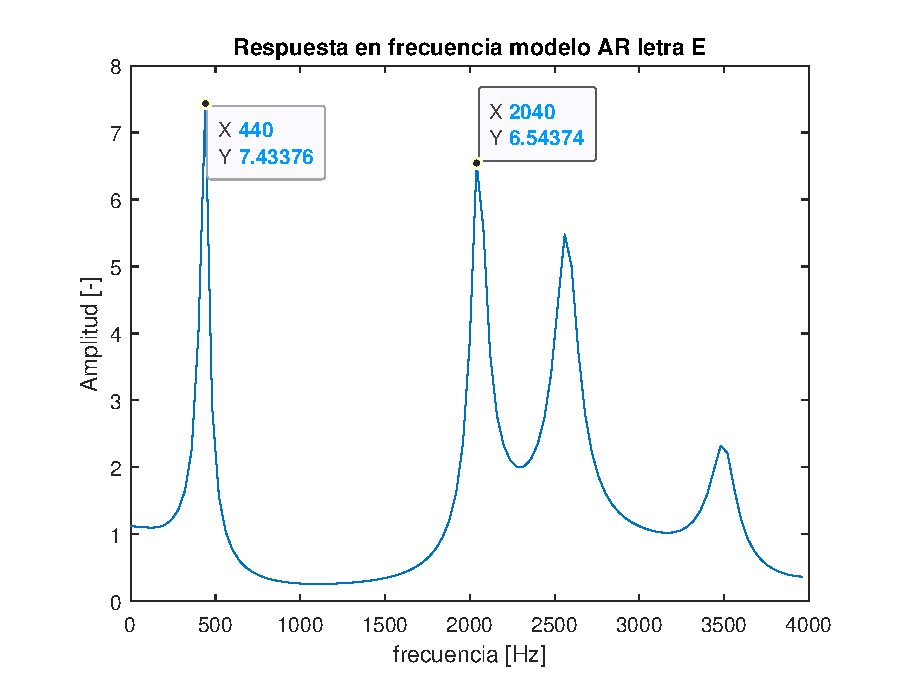
\includegraphics[width = .8\linewidth]{figures/p1_2e.eps}
    \caption{Respuesta en frecuencia de filtro estimado para simular tracto vocal haciendo letra e. Se destaca el primer y segundo formante encontrado.}
    \label{fig:p1_2e}
\end{figure}

\begin{figure}[H]
    \centering
    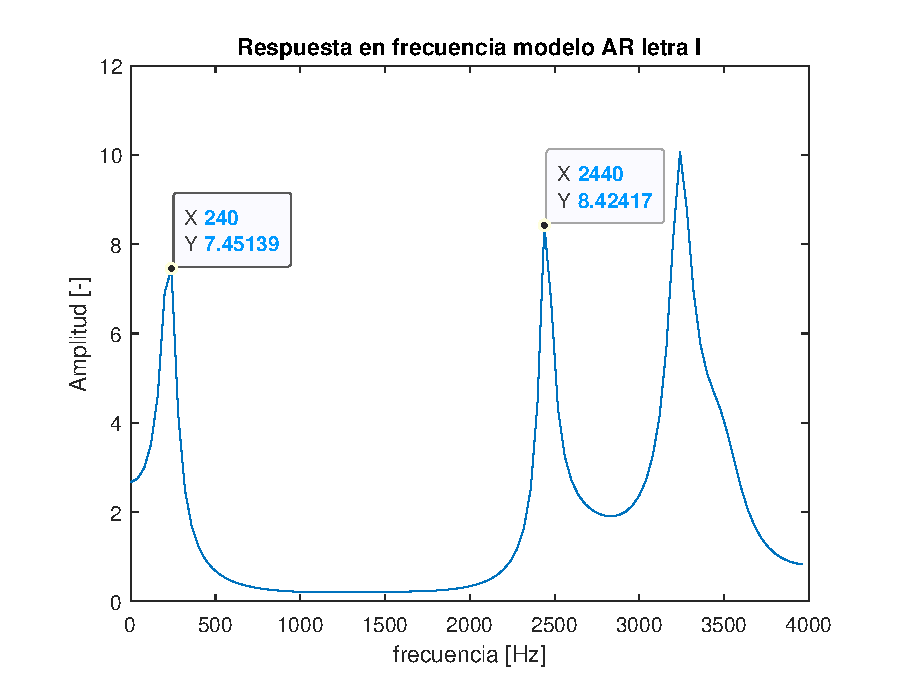
\includegraphics[width = .8\linewidth]{figures/p1_2i.eps}
    \caption{Respuesta en frecuencia de filtro estimado para simular tracto vocal haciendo letra i. Se destaca el primer y segundo formante encontrado.}
    \label{fig:p1_2i}
\end{figure}

\begin{figure}[H]
    \centering
    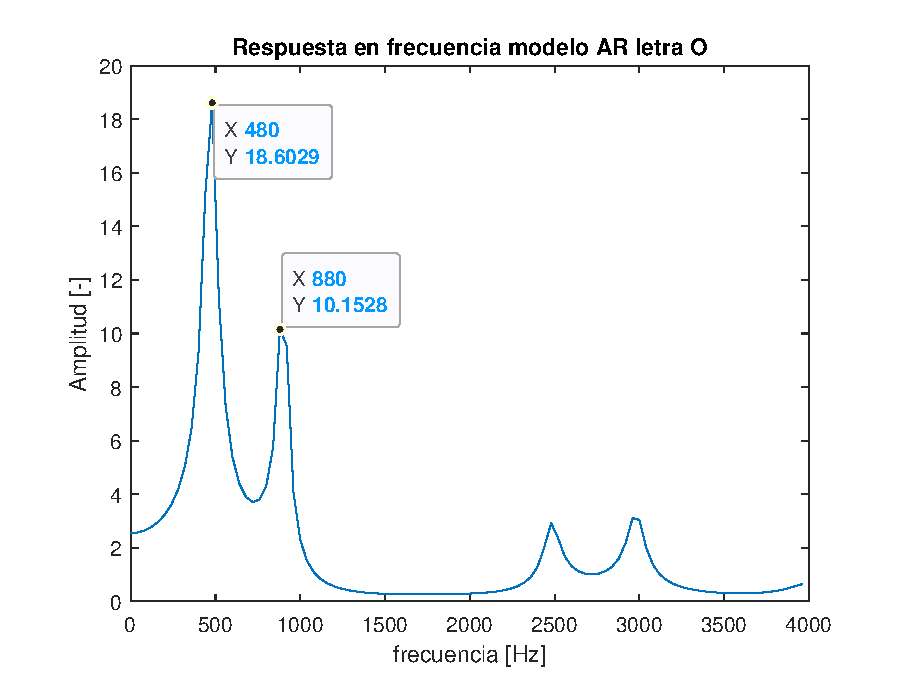
\includegraphics[width = .8\linewidth]{figures/p1_2o.eps}
    \caption{Respuesta en frecuencia de filtro estimado para simular tracto vocal haciendo letra o. Se destaca el primer y segundo formante encontrado.}
    \label{fig:p1_2o}
\end{figure}

\begin{figure}[H]
    \centering
    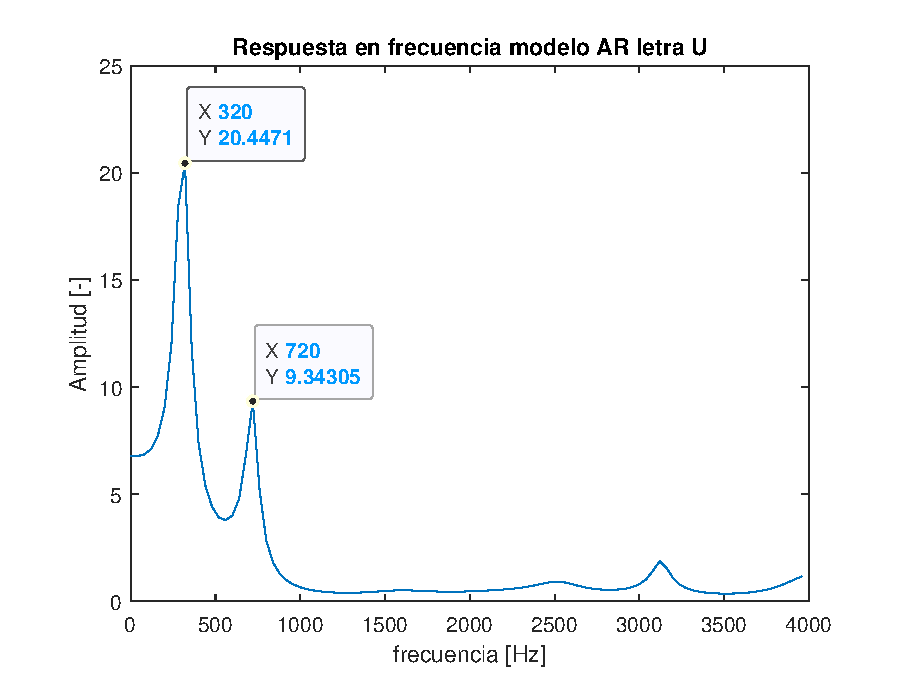
\includegraphics[width = .8\linewidth]{figures/p1_2u.eps}
    \caption{Respuesta en frecuencia de filtro estimado para simular tracto vocal haciendo letra u. Se destaca el primer y segundo formante encontrado.}
    \label{fig:p1_2u}
\end{figure}

De las figuras de las respuestas en frecuencia del tracto vocal por cada vocal se aprecia que los formantes de cada vocal están donde corresponden según el gráfico de formantes mostrado en la figura \ref{fig:p1_formantes}. Por otro lado en algunas vocales se aprecia un menor número de peaks, por lo que un valor menor de $P$ dependiendo la vocal podría ser suficiente (vocales i y u).

\begin{figure}[H]
    \centering
    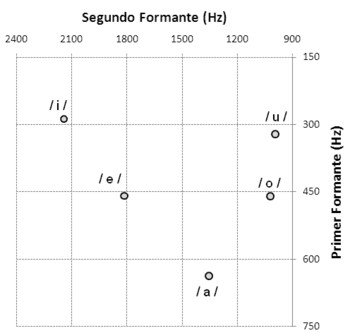
\includegraphics[width = .5\linewidth]{figures/350px-Spanish_Vowel_Formants_Bradlow1995.png}
    \caption{Gráfico de formantes de vocales en habla hispana.}
    \label{fig:p1_formantes}
\end{figure}

\subsection{Uso de filtros diseñados para síntesis de vocales}
Para esta sección se utiliza el código \texttt{p1\_3.m}, el cual se adjunta a la entrega.

Se utilizan los filtros AR diseñados en el punto anterior junto a la señal de tren impulsos generada en el parte 1.1 como entrada a los filtros para sintetizar archivos de audio.

La sección de código donde se genera la señal discreta que imita a un muestreo de una señal de audio de cada vocal se muestra a continuación:

\begin{lstlisting}
%%% 3. Generacion de archivos de audio (filtrado)
y_a = filter(1, a_vowel_a, x);
y_e = filter(1, a_vowel_e, x);
y_i = filter(1, a_vowel_i, x);
y_o = filter(1, a_vowel_o, x);
y_u = filter(1, a_vowel_u, x);
\end{lstlisting}

Con respecto a los archivos de audio generados, si es posible distinguir que vocal corresponde a cada una. Sobre la calidad de audio, todos los sonidos tienen un tono ''robótico'', siendo la letra u la que tiene menos calidad, al menos desde el parlante disponible al momento de escucharla. Las vocales se adjunta al informe en el formato \texttt{matlab\_vowel\_x} siendo \texttt{x} la vocal respectiva.

Para mejorar la calidad del audio se podría filtrar la señal generada con el sistema actual por un filtro pasa bajos a diseñar mediante algún criterio. Lo anterior se plantea debido a que se pueden percibir frecuencias altas en el audio que no son naturales en la voz humana a esa potencia. 

Los gráficos de los espectros en frecuencia de cada vocal sintetizada se muestran en las figuras \ref{fig:p1_3a} - \ref{fig:p1_3u}. Con respecto a las formas obtenidas, como era de esperarse, corresponden a un tren de impulsos con envolvente la respuesta en frecuencia del filtro de la vocal respectiva.

\begin{figure}[H]
    \centering
    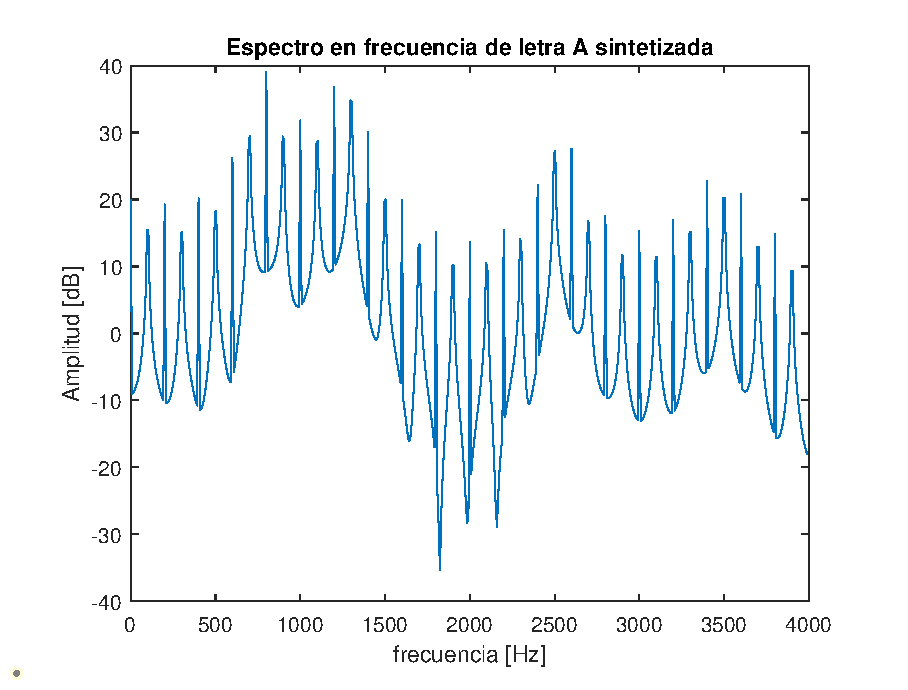
\includegraphics[width = .8\linewidth]{figures/p1_3a.eps}
    \caption{Espectro en frecuencia de letra A sintetizada.}
    \label{fig:p1_3a}
\end{figure}

\begin{figure}[H]
    \centering
    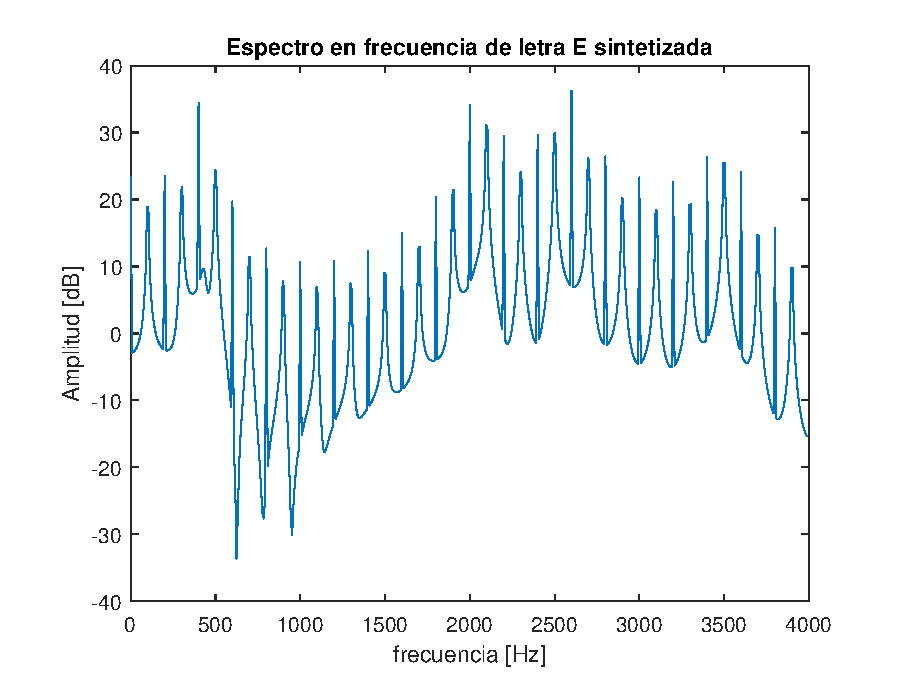
\includegraphics[width = .8\linewidth]{figures/p1_3e.eps}
    \caption{Espectro en frecuencia de letra E sintetizada.}
    \label{fig:p1_3e}
\end{figure}

\begin{figure}[H]
    \centering
    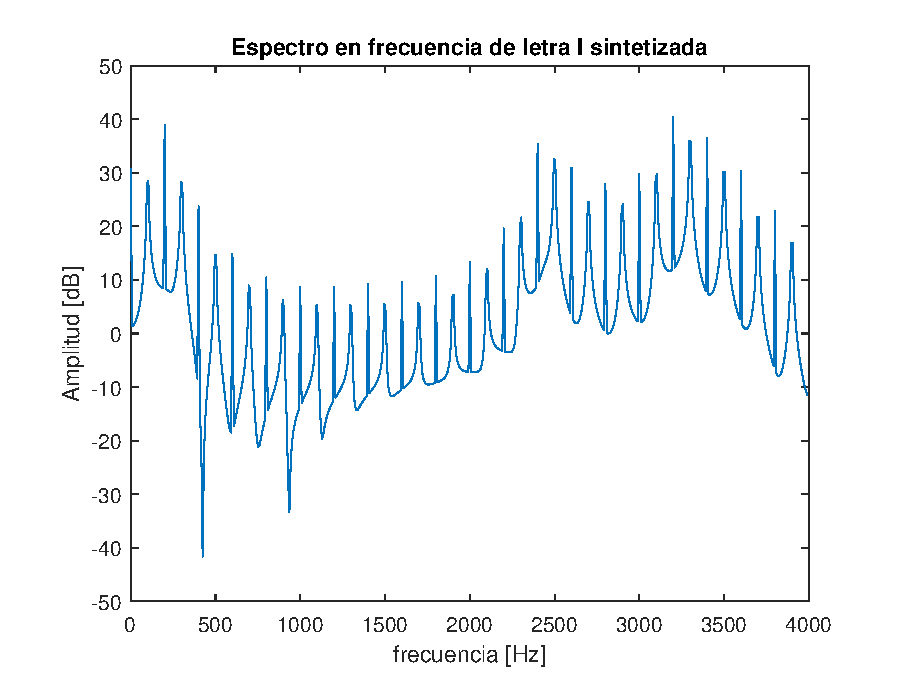
\includegraphics[width = .8\linewidth]{figures/p1_3i.eps}
    \caption{Espectro en frecuencia de letra I sintetizada.}
    \label{fig:p1_3i}
\end{figure}

\begin{figure}[H]
    \centering
    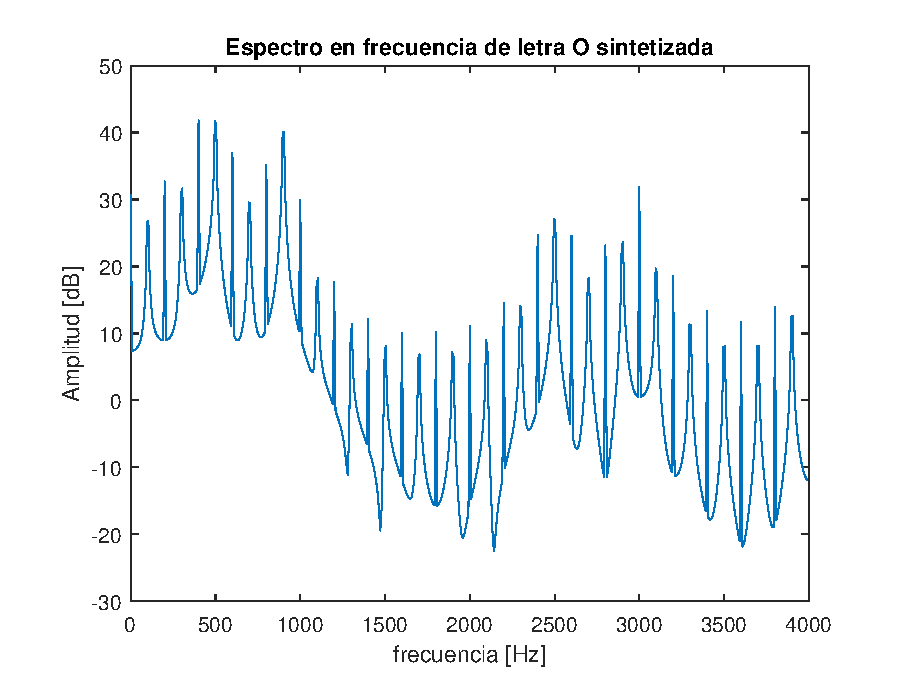
\includegraphics[width = .8\linewidth]{figures/p1_3o.eps}
    \caption{Espectro en frecuencia de letra O sintetizada.}
    \label{fig:p1_3o}
\end{figure}

\begin{figure}[H]
    \centering
    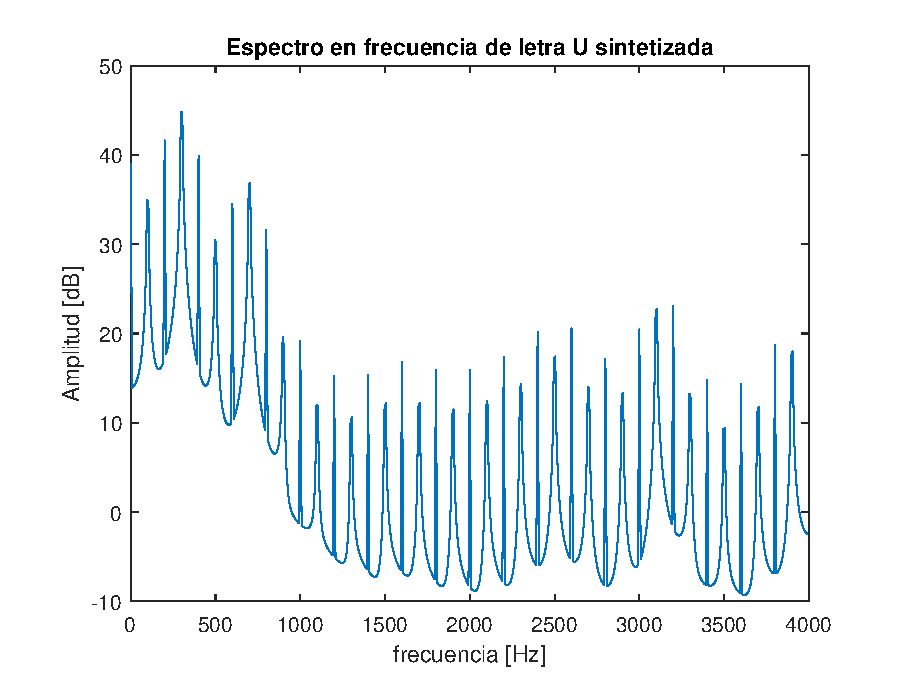
\includegraphics[width = .8\linewidth]{figures/p1_3u.eps}
    \caption{Espectro en frecuencia de letra U sintetizada.}
    \label{fig:p1_3u}
\end{figure}

\subsection{Generación de función $y = mylpc(x,p)$ y comparación con puntos anteriores}

En primer lugar se escribe la función $y=mylpc(x,p)$ la cual corresponde a una implementación del comando $lpc(x,p)$ usado anteriormente. El código se muestra a continuación:
\begin{lstlisting}[language = octave]
function y = mylpc(x,p)
    rx = xcorr(x);    
    rx_toeplitz  = rx(length(x):length(x)+p-1);
    rx = rx(length(x)+1:length(x)+p);

    Ra = toeplitz(rx_toeplitz);

    a = (Ra\rx)';
    y = [1 -a];
end
\end{lstlisting}

donde, obteniendo $R_x$ y $r_x$ a partir de estimaciones de la autocorrelación se resuelve $R_xa = r_x$, para finalmente retornar los parámetros del filtro AR diseñado.

Posteriormente se utiliza la nueva función para repetir los puntos 1.2 y 1.3. Los coeficientes AR obtenidos con el comando $lpc$ y $mylpc$ coinciden para cada vocal. Los gráficos de la respuesta en frecuencia de los filtros diseñados con $mylpc$ se muestran en las figuras \ref{fig:p1_4a} - \ref{fig:p1_4u}, coincidiendo con las obtenidas en 1.2.

Los archivos de audio resultantes se adjuntan a la entrega con el formato \texttt{mylpc\_vowel\_x} siendo \texttt{x} la vocal respectiva.

\begin{figure}[H]
    \centering
    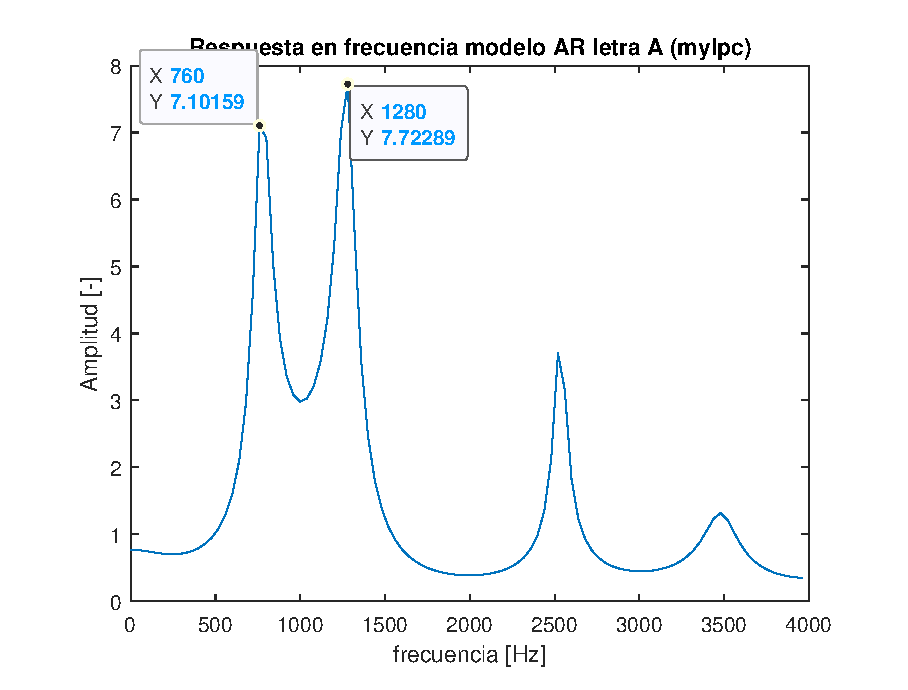
\includegraphics[width = .8\linewidth]{figures/p1_4a.eps}
    \caption{Respuesta en frecuencia de filtro estimado para simular tracto vocal haciendo letra a. Se destaca el primer y segundo formante encontrado ($mylpc$).}
    \label{fig:p1_4a}
\end{figure}

\begin{figure}[H]
    \centering
    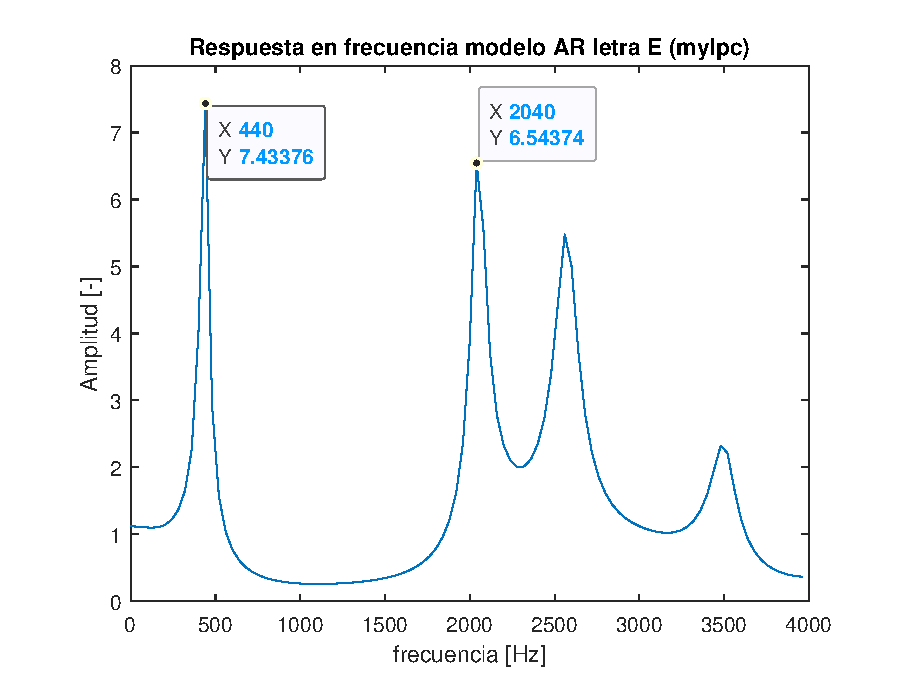
\includegraphics[width = .8\linewidth]{figures/p1_4e.eps}
    \caption{Respuesta en frecuencia de filtro estimado para simular tracto vocal haciendo letra e. Se destaca el primer y segundo formante encontrado ($mylpc$).}
    \label{fig:p1_4e}
\end{figure}

\begin{figure}[H]
    \centering
    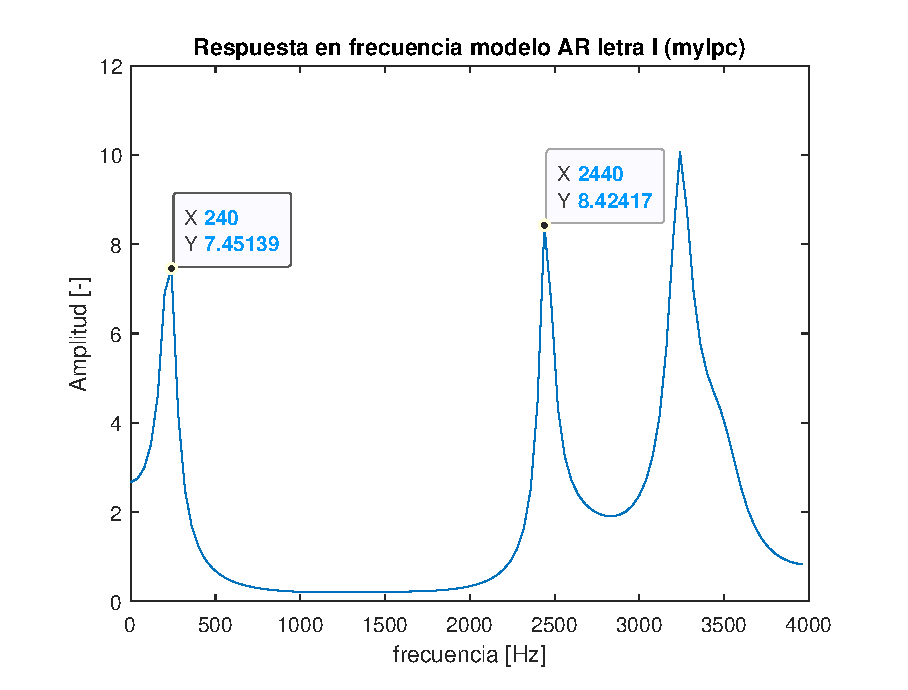
\includegraphics[width = .8\linewidth]{figures/p1_4i.eps}
    \caption{Respuesta en frecuencia de filtro estimado para simular tracto vocal haciendo letra i. Se destaca el primer y segundo formante encontrado ($mylpc$).}
    \label{fig:p1_4i}
\end{figure}

\begin{figure}[H]
    \centering
    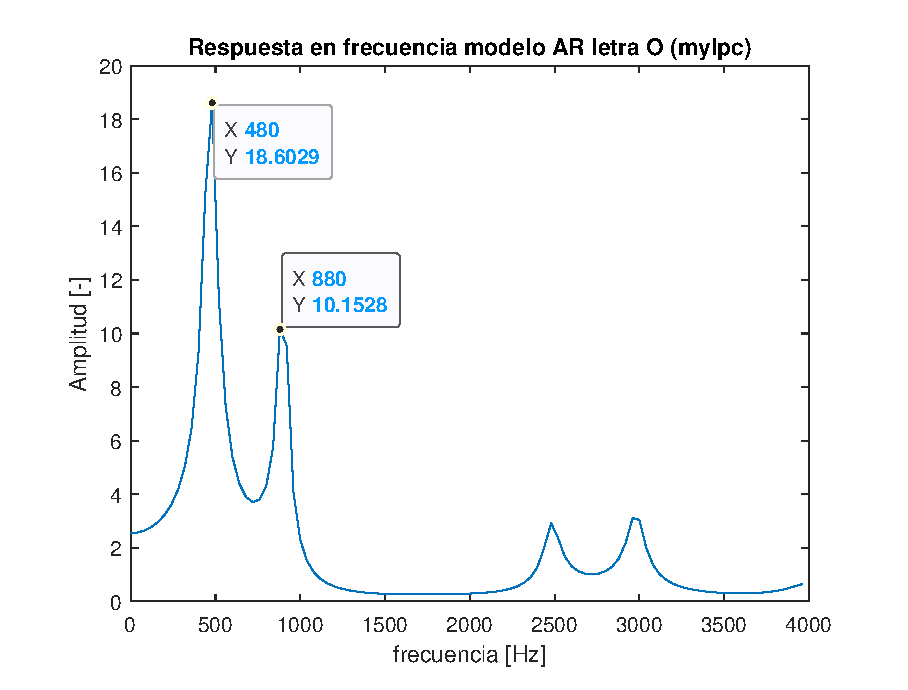
\includegraphics[width = .8\linewidth]{figures/p1_4o.eps}
    \caption{Respuesta en frecuencia de filtro estimado para simular tracto vocal haciendo letra o. Se destaca el primer y segundo formante encontrado ($mylpc$).}
    \label{fig:p1_4o}
\end{figure}

\begin{figure}[H]
    \centering
    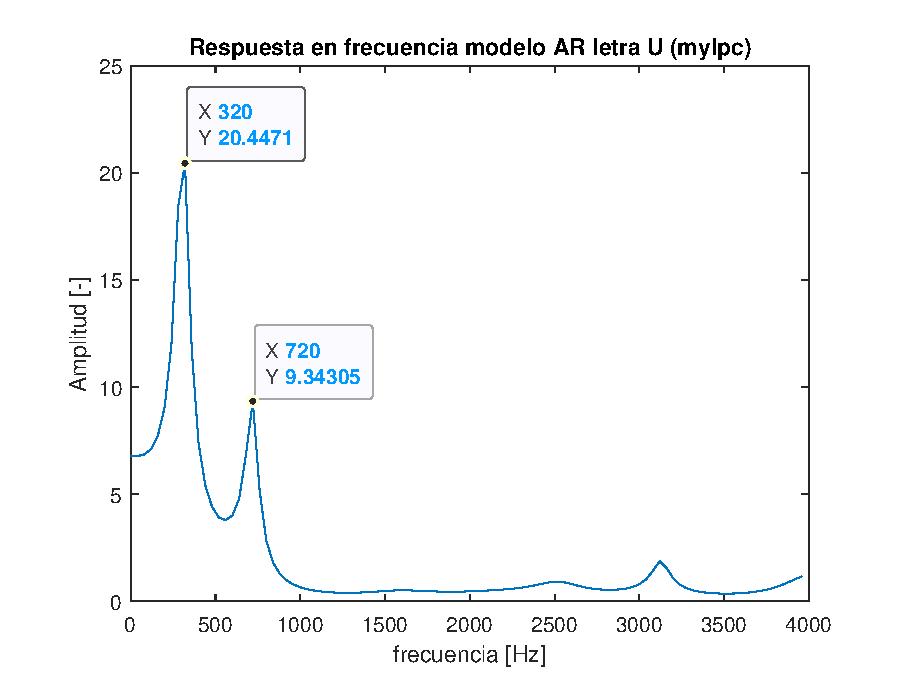
\includegraphics[width = .8\linewidth]{figures/p1_4u.eps}
    \caption{Respuesta en frecuencia de filtro estimado para simular tracto vocal haciendo letra u. Se destaca el primer y segundo formante encontrado ($mylpc$).}
    \label{fig:p1_4u}
\end{figure}





\clearpage

%II
\section{Clasificación de segmentos VUS}

Se pide escribir función que para obtener el número de cruces por cero por milisegundo de una señal. El código escrito se muestra a continuación:
\begin{lstlisting}[language = octave]
function n_ms = cruces_zero(x,fs)
    n = 0;
    
    for i = 1:length(x)-1
        if x(i+1)*x(i) < 0
            n = n+1;
        end
    end
    
    ms = 1000*length(x)/fs;
    n_ms = n/ms;    
end
\end{lstlisting}

\subsection{Obtención de Criterios de Clasificación}

Para esta sección se utiliza el código \texttt{p2\_1.m}, el cual se adjunta a la entrega.

En primer primer lugar se separa la señal $training\_signal$ por cada letra con la ayuda del comando $ginput$. Esta señal corresponde a alguien diciendo ''señales temporales''. La separación se muestra en la figura \ref{fig:p2_1clas}
\begin{figure}[H]
    \centering
    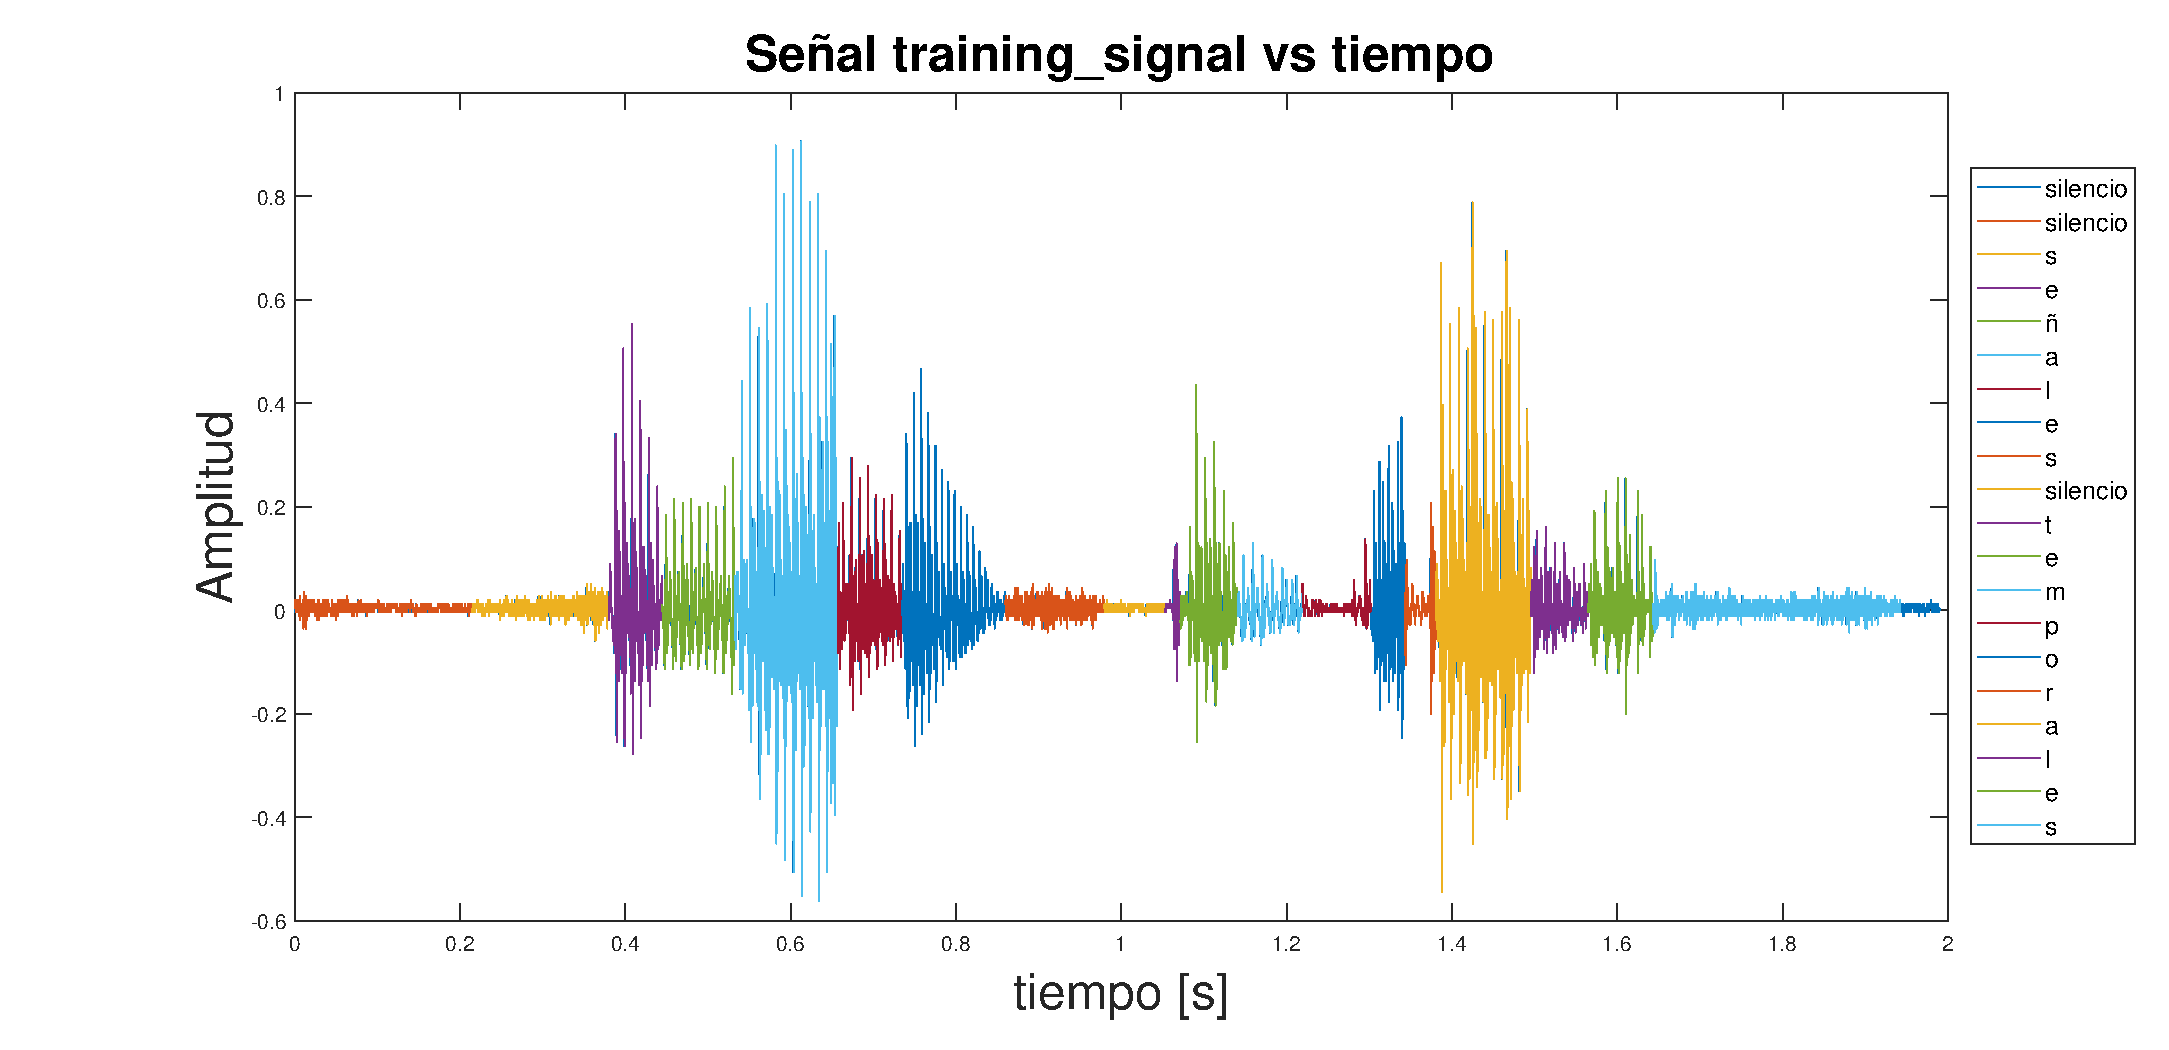
\includegraphics[width = .9\linewidth]{figures/p2_1separacion.eps}
    \caption{Separación manual por cada letra y silencios en señal $training\_signal$.}
    \label{fig:p2_1clas}
\end{figure}

En el cuadro \ref{tab:p2_1tab} se muestra el valor RMS, la razón de Cruces por Cero por milisegundo y la clasificación VUS de los segmentos encontrados en $training\_signal$.

\begin{table}[H]
    \centering
    \begin{tabular}{c|c|c|c}
        Sonido & RMS & Ratio Cruces por Cero & Clasificación VUS  \\ \hline
        Silencio 1    &0.0077     &2.7242 &S\\
        s             &0.0121     &3.8855 &U\\
        e             &0.0995     &1.6557 &V\\
        ñ             &0.0766     &1.0613 &U\\
        a             &0.1617     &2.9960 &V\\
        l             &0.0685     &2.3987 &U\\
        e             &0.0788     &1.5984 &V\\
        s             &0.0151     &4.5381 &U\\
        Silencio 2    &0.0061     &2.4678 &S\\
        t             &0.0359     &1.7297 &U\\
        e             &0.0714     &1.4756 &V\\
        m             &0.0336     &0.8166 &U\\
        p             &0.0161     &2.0000 &U\\
        o             &0.0911     &1.5181 &V\\
        r             &0.0394     &1.7627 &U\\
        a             &0.1525     &1.9349 &V\\
        l             &0.0412     &1.4611 &U\\
        e             &0.0544     &1.9904 &V\\
        s             &0.0136     &4.3554 &U\\
        Silencio 3    &0.0061     &2.4632 &S
    \end{tabular}
    \caption{Valor RMS, Ratio de Cruces por Cero por milisegundo y Clasificación VUS de segmentos encontrados en $training\_signal$}
    \label{tab:p2_1tab}
\end{table}

Posteriormente se obtiene una nube de puntos para los segmentos VUS, donde el eje horizontal corresponde al valor RMS y el vertical a los cruces por cero. Dicho gráfico se muestra en la figura \ref{fig:p2_1nube}.

\begin{figure}[H]
    \centering
    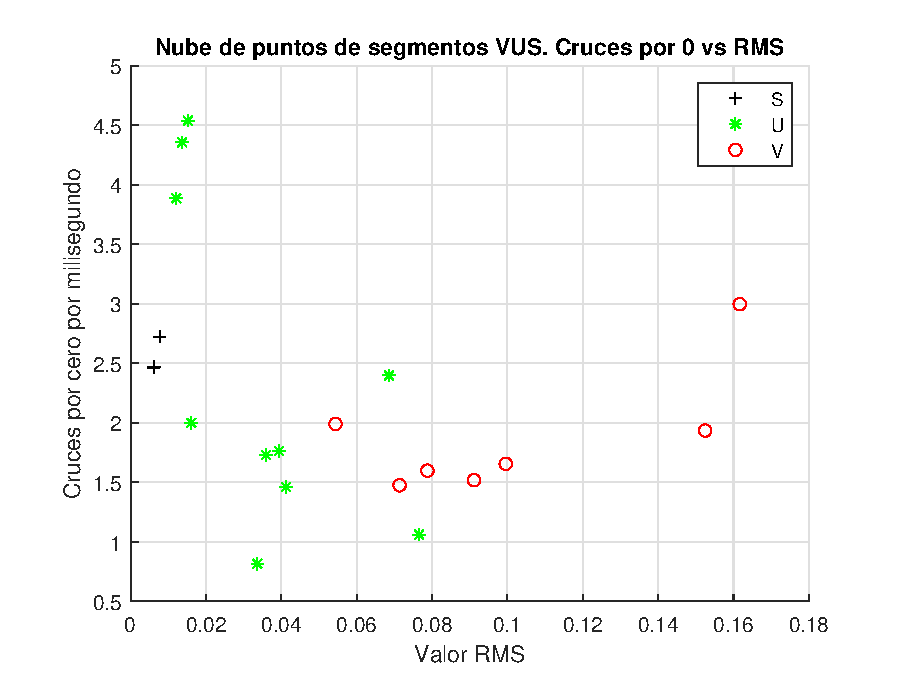
\includegraphics[width = .8\linewidth]{figures/p2_1nube.eps}
    \caption{Nube de puntos para los segmentos VUS para una posterior clasificación.}
    \label{fig:p2_1nube}
\end{figure}

A partir de la nube de puntos y una inspección visual sencilla se concluyen los siguientes criterios de clasificación:
\begin{enumerate}
    \item Valor RMS:
    \begin{itemize}
        \item Si $RMS < 0.01$: Sonido tipo S.
        \item Si $0.01 \leq RMS < 0.06$: Sonido tipo U.
        \item Si $RMS \geq 0.06$: Sonido tipo V.
    \end{itemize}
    
    \item Cruces por cero ($CZ$):
    \begin{itemize}
        \item Si $CZ < 2.25$: Sonido tipo V.
        \item Si $2.25 \leq CZ < 2.8$: Sonido tipo S.
        \item Si $CZ \geq 2.8$: Sonido tipo U.
    \end{itemize}
\end{enumerate}

Viendo la nube de puntos la decisión de clasificar los segmentos mediante umbrales en los cruces por cero no parece ser un método muy fiable. Por otro lado, umbrales en el valor RMS parece tener un mejor desempeño con respecto a la clasificación.

%%%%%%%%%%%%%%%%%%%%%%%%%%%%%%%%%%%%%%%%%%%%%%%%%%%%%%%%%%%5
\subsection{Comparación de criterios}

Para esta sección se utiliza el código \texttt{p2\_2.m}, el cual se adjunta a la entrega.

Cómo método combinado se propone:
\begin{enumerate}
    \item Valor RMS y Cruces por Cero ($CZ$):
    \begin{itemize}
        \item Si $CZ < -250RMS + 5$: Sonido tipo S.
        \item Si $CZ \geq -250RMS + 5$ y $RMS < 0.06$: Sonido tipo U.
        \item Si $RMS \geq 0.06$: Sonido tipo V.
    \end{itemize}
\end{enumerate}
El cual se obtuvo a partir de delimitar la nube de puntos obtenida en la sección anterior por 2 rectas, las cuales se muestran en la figura \ref{fig:p2_2nube}.

\begin{figure}[H]
    \centering
    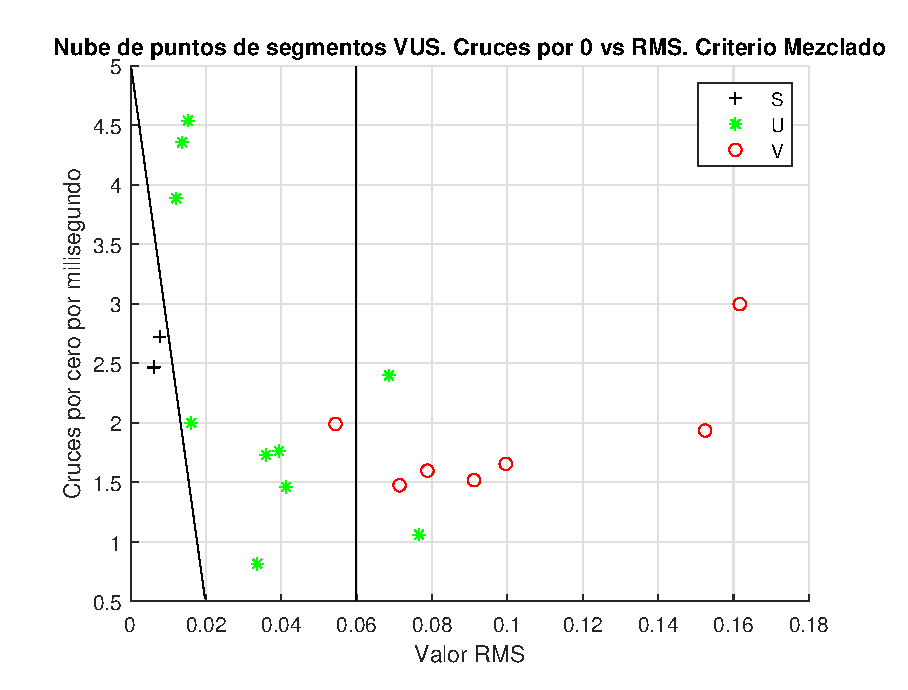
\includegraphics[width = .8\linewidth]{figures/p2_2nube.eps}
    \caption{Nube de puntos para los segmentos VUS con rectas para clasificación con criterio combinado.}
    \label{fig:p2_2nube}
\end{figure}

Al revisar los resultados de los 3 métodos, se aprecia que:
\begin{itemize}
    \item El criterio de los Cruces por Cero presenta resultados no satisfactorios. Lo anterior era esperable debido a que no se apreciaba una correlación en la nube de puntos lo suficientemente fuerte como para aplicar umbrales.
    \item El criterio del valor RMS presenta resultados bastante mejores que el de cruces por cero. De la nube de puntos era esperable que umbrales en el valor RMS (separación del plano por líneas verticales) debía dar mejores resultados en la clasificación.
    \item El criterio combinado propuesto entrega resultados muy similares de clasificación de puntos. Lo anterior no es una sorpresa, ya que este criterio puede interpretarse como una leve inclinación de la recta vertical correspondiente al umbral más bajo del criterio RMS.
\end{itemize}

Por todo lo anterior se concluye que desde una perspectiva costo-efectivo el mejor criterio encontrado corresponde al del valor RMS. 

%Debiese haber un parrafo donde propongas el método combinado (puede ser también por umbrales y alguna combinación lineal). Con que sea al ojo cualquier cosa mas o menos lógica está bien. Te puedes justificar en función a la nube de puntos de la figura p2_1nube

% Tienes que implementar el método en matlab. usa umbrales nomás y sera copiar y pegar código que ya está en el p2_2.m.

%Tiene que haber un segundo párrafo donde comentes como anduvieron estos 3 métodos. El de cruces por cero es re malo así que al final será comparar el RMS con el propuesto por tí y probablemente se concluya que el mejor en terminos costo-efectividad sea el criterio RMS.


%%%%%%
Finalmente se grafica la señal $text\_signal$, la variable VUS (1, -1 o 0) obtenida a partir de la estimación de RMS y el valor RMS de los segmentos. Dichos gráficos se muestran en la figura \ref{fig:p2_2grafs}. Con respecto a los gráficos se puede comentar que:
\begin{itemize}
    \item Como es de esperarse, el valor RMS se comporta como una especie de envolvente de la señal.
    \item Al ser la señal ''sonidos de voz'' es claro que el criterio presenta falencias en la clasificación.
    \item A partir de la evolución del valor RMS en el tiempo, podría mejorar la clasificación cambiando los umbrales.
\end{itemize}

\begin{figure}[H]
    \centering
    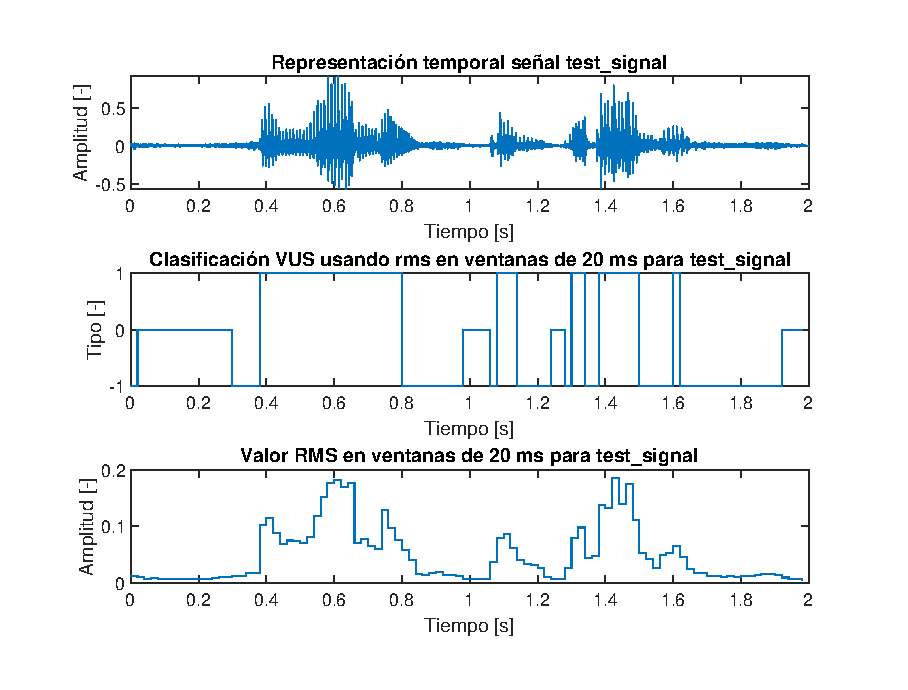
\includegraphics[width = .9\linewidth]{figures/p2_2grafs.eps}
    \caption{Señal $text\_signal$, clasificación VUS (RMS) y valor RMS de segmentos clasificados.}
    \label{fig:p2_2grafs}
\end{figure}








\clearpage

%III
\section{Síntesis de voz hablada}


\subsection{Compresión y Síntesis de Señal de Voz}

Se pide aplicar compresión y síntesis la señal de voz $test\_signal$. Los pasos para realizar lo anterior corresponden a:
\begin{itemize}
    \item Compresión:
    \begin{enumerate}
        \item Subdividir la señal en segmentos de 20 ms.
        \item Obtener el valor RMS de cada segmento.
        \item Clasificar cada segmento como V, U o S con el criterio basado en RMS obtenido en la parte 2.
        \item Obtener los valores del filtro AR que simula el tracto vocal por medio de $mylpc$ para los sonidos de tipo V y U.
    \end{enumerate}
    \item Síntesis:
    
    Se van generando los segmentos en orden
    \begin{itemize}
        \item En el caso de que un segmento corresponda a un sonido S, generar segmento de silencio (ceros) de 20 ms.
        \item En el caso de que el sonido corresponda a un sonido V, excitar filtro AR respectivo con tren de impulsos de 20 ms (en este caso de 100 Hz).  Realizar corrección de RMS del segmento.
        \item En el caso de que el sonido corresponda a un sonido U, excitar filtro AR respectivo con señal de ruido blanco de 20 ms.  Realizar corrección de RMS del segmento.
    \end{itemize}
    Finalmente se concatenan los segmentos generados
\end{itemize}

El código que realiza lo anterior corresponde a \texttt{p3\_1.m} y se adjunta a la entrega.
 
El gráfico de la señal original y la sintetizada se muestran en la figura \ref{fig:p3_1}. Visualmente la síntesis parece correcta.

\begin{figure}[H]
    \centering
    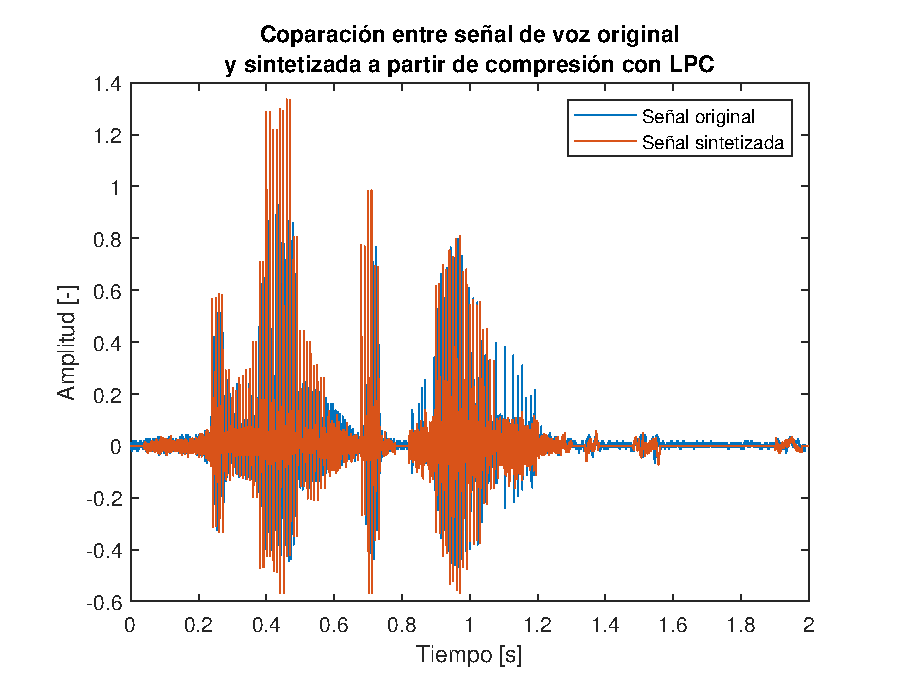
\includegraphics[width = .9\linewidth]{figures/p3_1.eps}
    \caption{Comparación gráfica de señal de voz original y sintetizada.}
    \label{fig:p3_1}
\end{figure}

Finalmente se guarda la señal sintetizada como $my\_test\_signal.wav$, la cual se adjunta a la entrega. Con respecto a la calidad del audio, si bien mantiene el timbre ''robótico'', se entiende lo que se esta diciendo. 

Para mejorar la síntesis se podría reconocer la frecuencia fundamental de la voz en sonidos tipo V y U, con la idea de excitar el filtro AR con un tren de impulsos de frecuencia acorde al hablante, obteniendo una voz más natural.

\subsection{Estimación de Compresión}

Se estima la compresión del archivo de audio como la razón entre los bytes usados para almacenar los coeficientes del filtro, los flags VUS y el valor RMS con respecto a los bytes de la señal $test\_signal$. Para lo anterior se utilizó el comando $whos$

Por lo tanto, la razón de compresión $R$ corresponde a:
$$ R = \dfrac{\text{bytes}(A) + \text{bytes}(flags) + \text{bytes}(RMSs)} {\text{bytes}(test\_signal)} = \dfrac{9088 + 100 + 100}{127360} \approx  0.079$$
\clearpage

%IV
\section{Filtro AR}

\subsection{Función \textit{positiveSpectrum}}

Se implementa la función \textit{positiveSpectrum(x)} que recibe como entrada una señal digital \textit{x}, de largo $N$, la cual haciendo uso de la función \textit{fft()}  de Matlab pueda entregar el vector \textit{amp} que corresponde  de amplitudes de la DFT  para el rango de frecuencias positivas y un vector \textit{w} correspondiente a las frecuencias normalizadas en \textit{rad/muestra}. El código de la función descrita se presenta a continuación


\begin{lstlisting}[language = octave]
function [amp,w] = positiveSpectrum(x)
    X = fft(x);
    amp = X(1:floor(length(X)/2))
    w = linspace(0,pi,length(amp))
end

\end{lstlisting}

Para poner a prueba la función implementada se grafica usando el comando  \texttt{plot()} el espectro en frecuencia positivo de la vocal \textit{A} contenida en la señal \textit{vowel\_a}, obteniendo la gráfica presente en la figura \ref{frec_A_positive}

\begin{figure}[H]
    \centering
    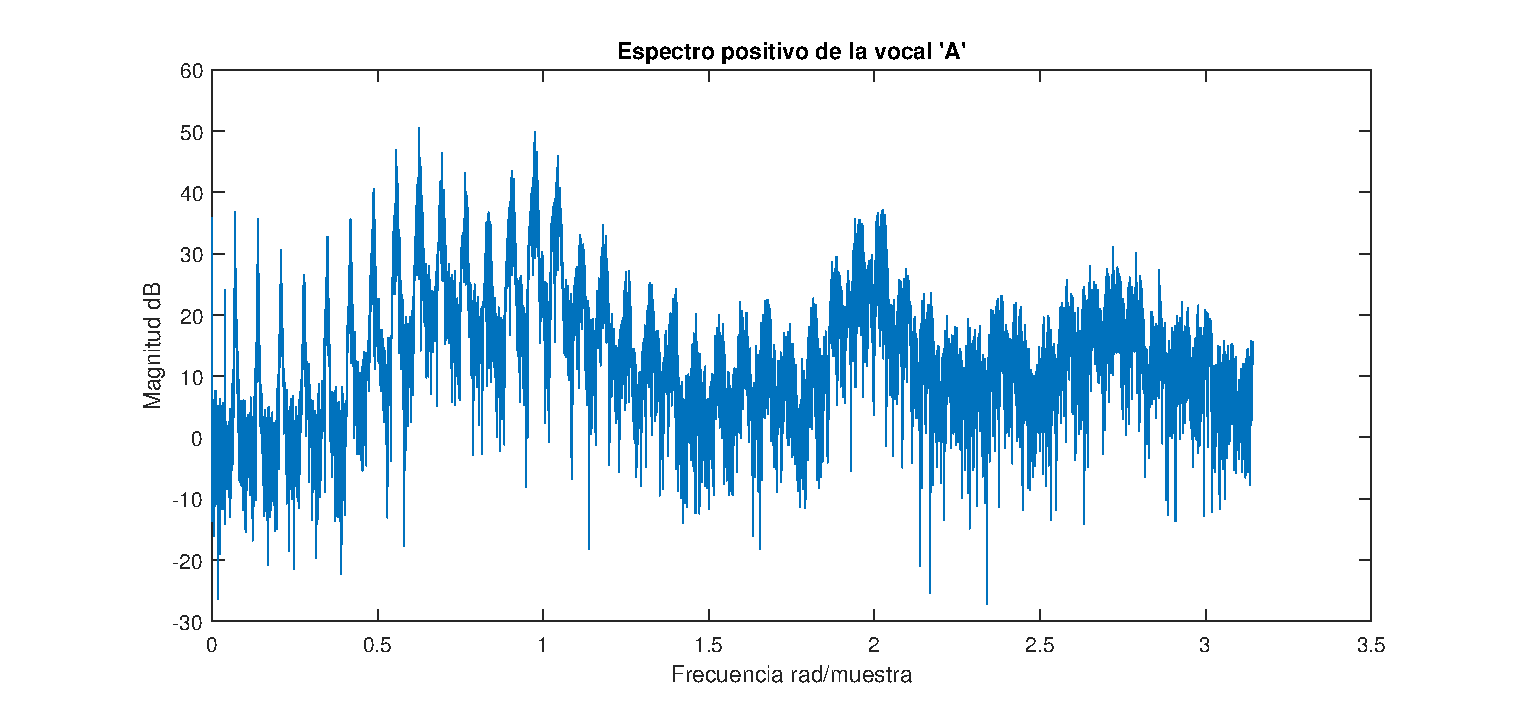
\includegraphics[scale = 0.5]{figures/4_1_espectroA.eps}
    \caption{Espectro de la señal \textit{vowel\_a}}
    \label{frec_A_positive}
\end{figure}

En el espectro obtenido se pueden diferenciar 4 formantes ubicadas aproximadamente en $0.6$, $1.2$, $2$ y $2.7 ~rad/muestra$ 
\subsection{Experimentación con Órdenes del filtro AR en LPC}

Para está parte se utiliza el código \texttt{p4\_2.m}, el cual se adjunta a la entrega.

Inicialmente se gráfica de la respuesta en frecuencia del filtro AR de orden 15 y 2, junto al espectro de $vowel\_a$. Los gráficos se muestran en la figura \ref{fig:p4_21}. Se aprecia que con 2 polos se tiende a formar una resonancia al medio de los 2 formantes de la vocal. 

\begin{figure}[H]
    \centering
    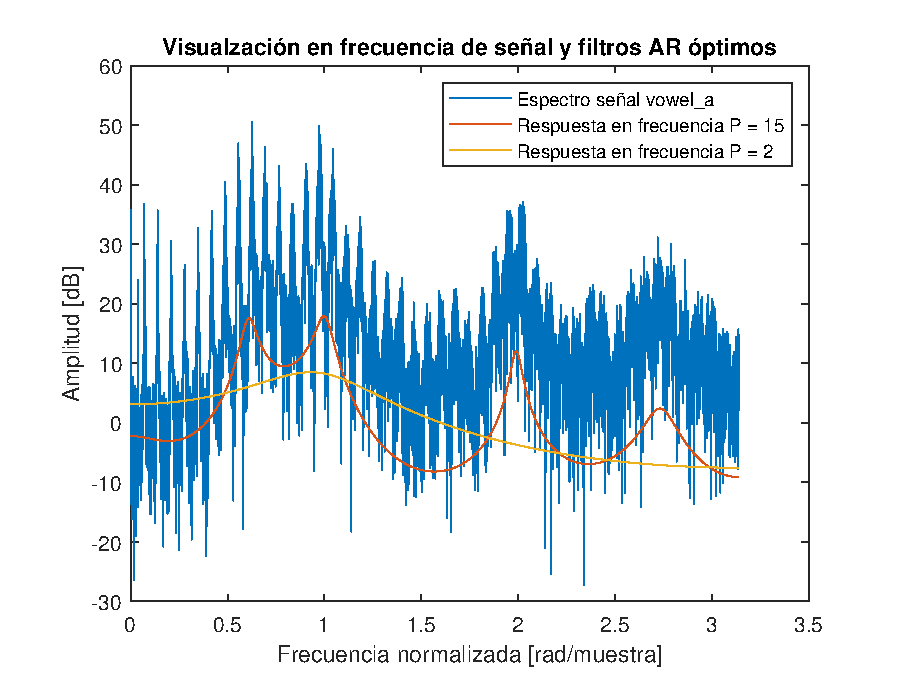
\includegraphics[width = .8\linewidth]{figures/p4_2arbajo.eps}
    \caption{Espectro de $vowel\_a$ y respuesta en frecuencia del filtro AR de orden 15 y 2 obtenidos por LPC.}
    \label{fig:p4_21}
\end{figure}

Por otro lado se obtiene el diagrama de polos y ceros de los filtros diseñados para la vocal a. Dichos diagramas se muestran en la figura \ref{fig:p4_22}

\begin{figure}[H]
    \centering
    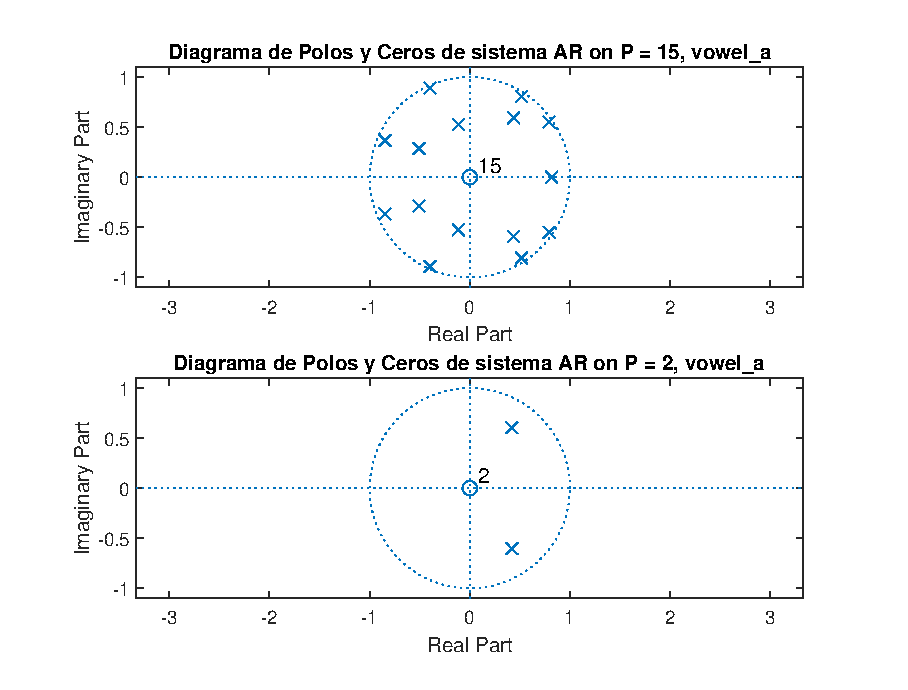
\includegraphics[width = .8\linewidth]{figures/p4_22.eps}
    \caption{Diagrama de polos y ceros para filtros de orden 15 y 2 diseñados por LPC para la señal $vowel\_a$.}
    \label{fig:p4_22}
\end{figure}

Posteriormente se grafica de la respuesta en frecuencia del filtro AR de orden 15 y 2, junto al espectro de $vowel\_u$, los cuales se muestran en la figura \ref{fig:p4_23}. Se aprecia que con 2 polos se tiende a formar una resonancia en la frecuencia 0. Lo anterior también se aprecia en la figura \ref{fig:p4_24}, donde se presenta el diagrama de polos y ceros para los filtros diseñados para la vocal u.

\begin{figure}[H]
    \centering
    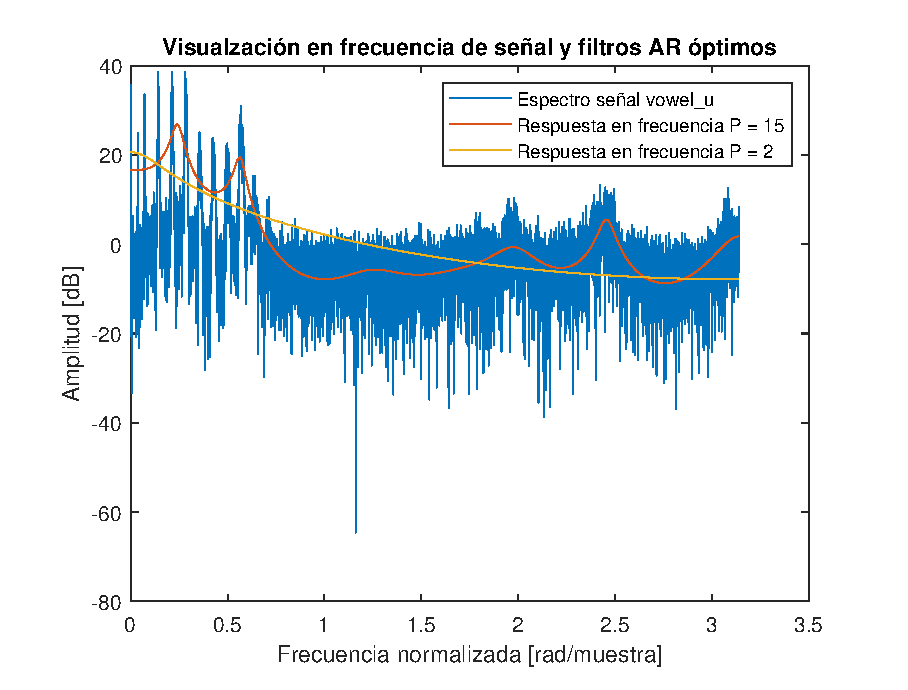
\includegraphics[width = .8\linewidth]{figures/p4_23.eps}
    \caption{Espectro de $vowel\_u$ y respuesta en frecuencia del filtro AR de orden 15 y 2 obtenidos por LPC.}
    \label{fig:p4_23}
\end{figure}

\begin{figure}[H]
    \centering
    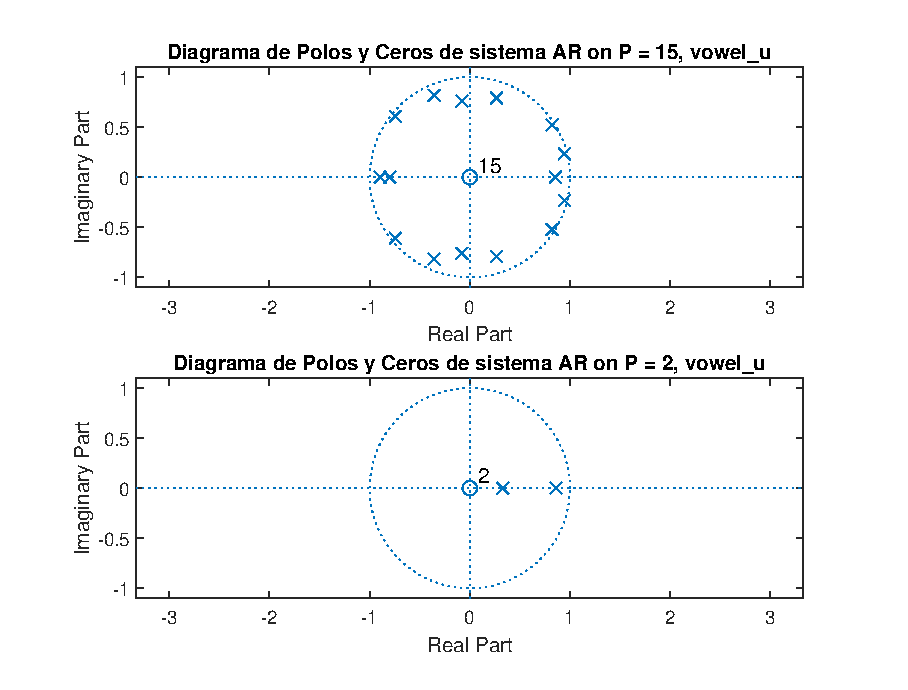
\includegraphics[width = .8\linewidth]{figures/p4_24.eps}
    \caption{Diagrama de polos y ceros para filtros de orden 15 y 2 diseñados por LPC para la señal $vowel\_u$.}
    \label{fig:p4_24}
\end{figure}



%%%%%%%%%%%%%%%%%%%%%%%%%%%%%%%%%%%%%%%%%%%%%%%%%%%%%%%%%%%%
\subsection{Comparación de filtrado AR de distinto orden}

Para estudiar las diferencias de resultados al filtrar una señal con filtros AR de distinto orden, primero se escoge una señal de vocal arbitraria para que sea filtrada, en este caso se escogió la señal \textit{vowel\_a} correspondiente a la vocal \textit{A}.

Lo siguiente es definir los ordenes de los filtros que se usarán, se escoge como referencia un orden relativamente alto 15 y uno menos de 9. Se crea un tren de impulsos de $100~Hz$ de frecuencia  con $0.5~s$ de duración. Se obtienen los coeficientes $a_k$ de cada filtro y se procede con el filtrado de la señal.

Los resultados obtenidos se muestran en las gráficas de la figura \ref{AR-15-9}, se incluyen además los diagramas de polos y ceros en la figura \ref{zplane1}, donde la gráfica superior corresponde al diagrama asociado al filtro de orden 15 y la inferior al filtro de orden 9.


\begin{figure}[H]
    \centering
    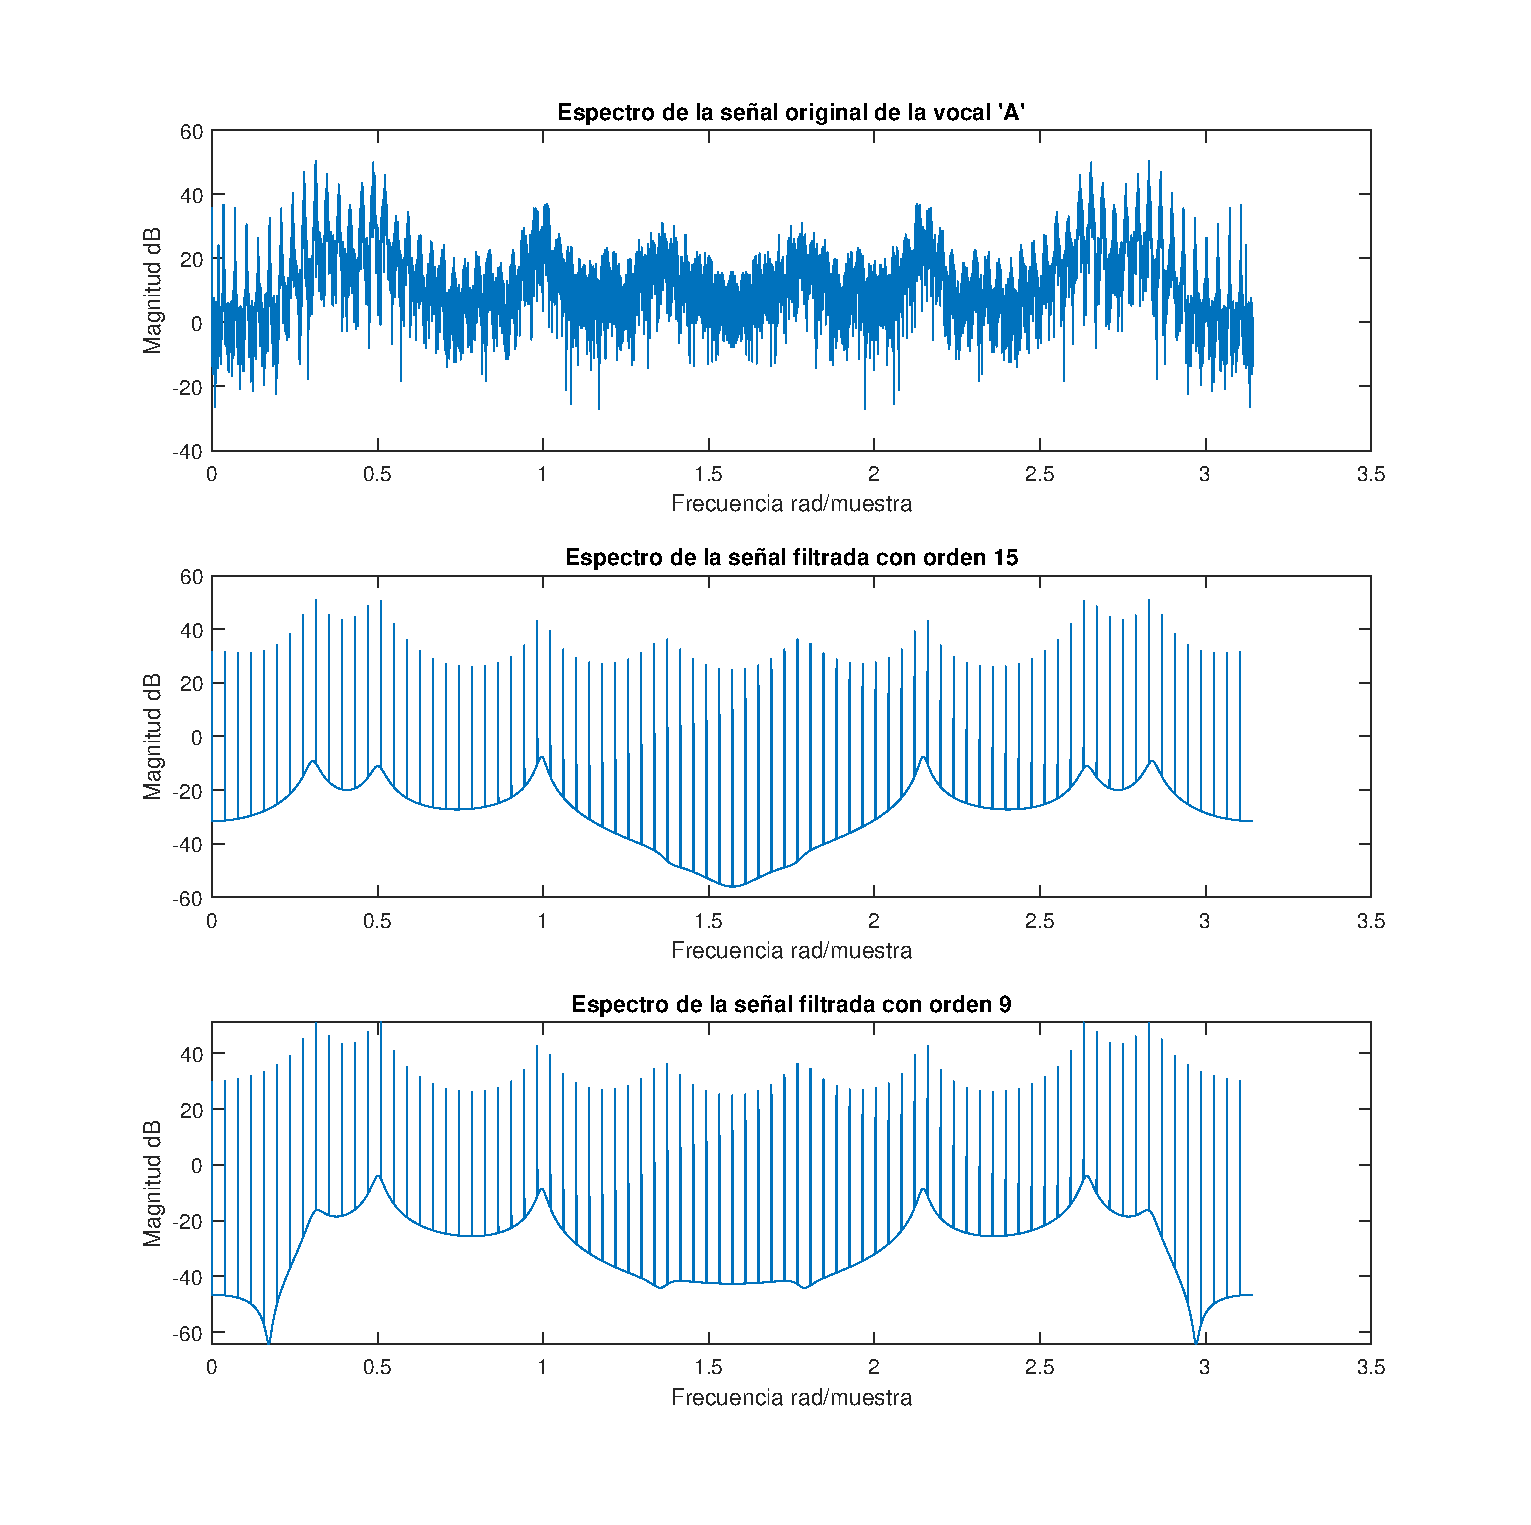
\includegraphics[scale = 0.6]{figures/4_3_filtradoAR.eps}
    \caption{Espectro en frecuencia de la señal \textit{vowels\_a} y el resultado de filtrado de orden 15 y 9 }
    \label{AR-15-9}
\end{figure}

\begin{figure}[H]
    \centering
    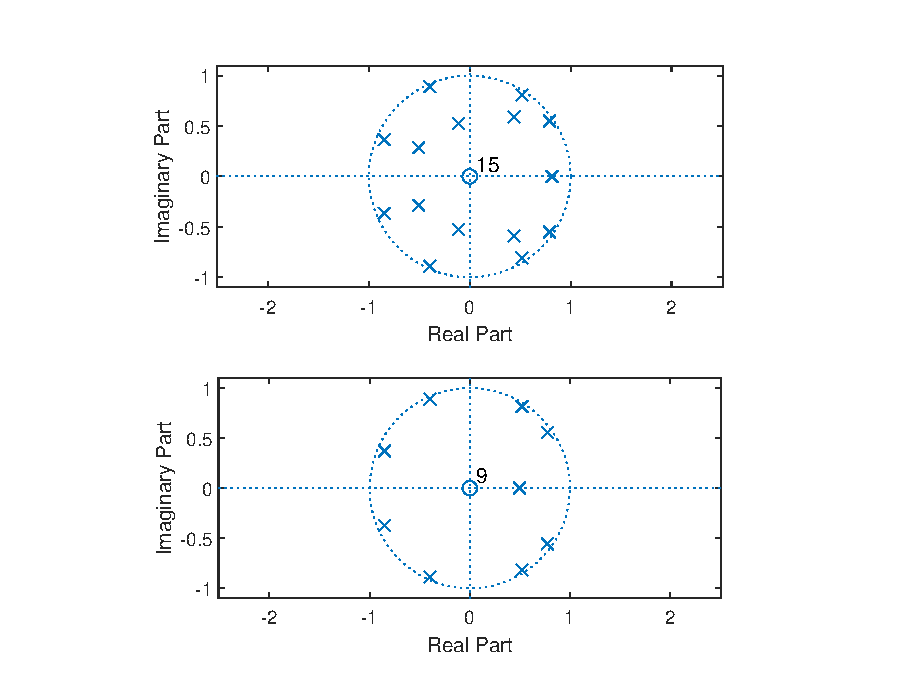
\includegraphics[scale = 0.9]{figures/4_3_zplane1.eps}
    \caption{Diagramas de polos y ceros para los filtros AR de orden 15 y 9}
    \label{zplane1}
\end{figure}


Se pide además realizar el mismo ejercicio anterior comparando el filtrado de la señal \textit{vowel\_u} correspondiente a la vocal \textit{U}, probando distintos ordenes de filtrado hasta encontrar el mínimo orden que no presente diferencias significativas en cuando a la percepción auditiva  respecto al resultado obtenido con el filtrado de orden 15. 

Se notó que haciendo uso de un filtro de orden 10 la señal ya se distorsiona lo suficiente para tener la impresión de que la vocal está siendo emitida por una persona distinta, por lo que se concluye que el orden mínimo para no tener diferencias significativas un filtro de orden 11. Los espectros en frecuencia obtenidos para filtros de orden 15 y 10 se presentan en la figura \ref{AR-15-10},  se incluyen además los diagramas de polos y ceros en la figura \ref{zplane2}, donde la gráfica superior corresponde al diagrama asociado al filtro de orden 15 y la inferior al filtro de orden 10.

\begin{figure}[H]
    \centering
    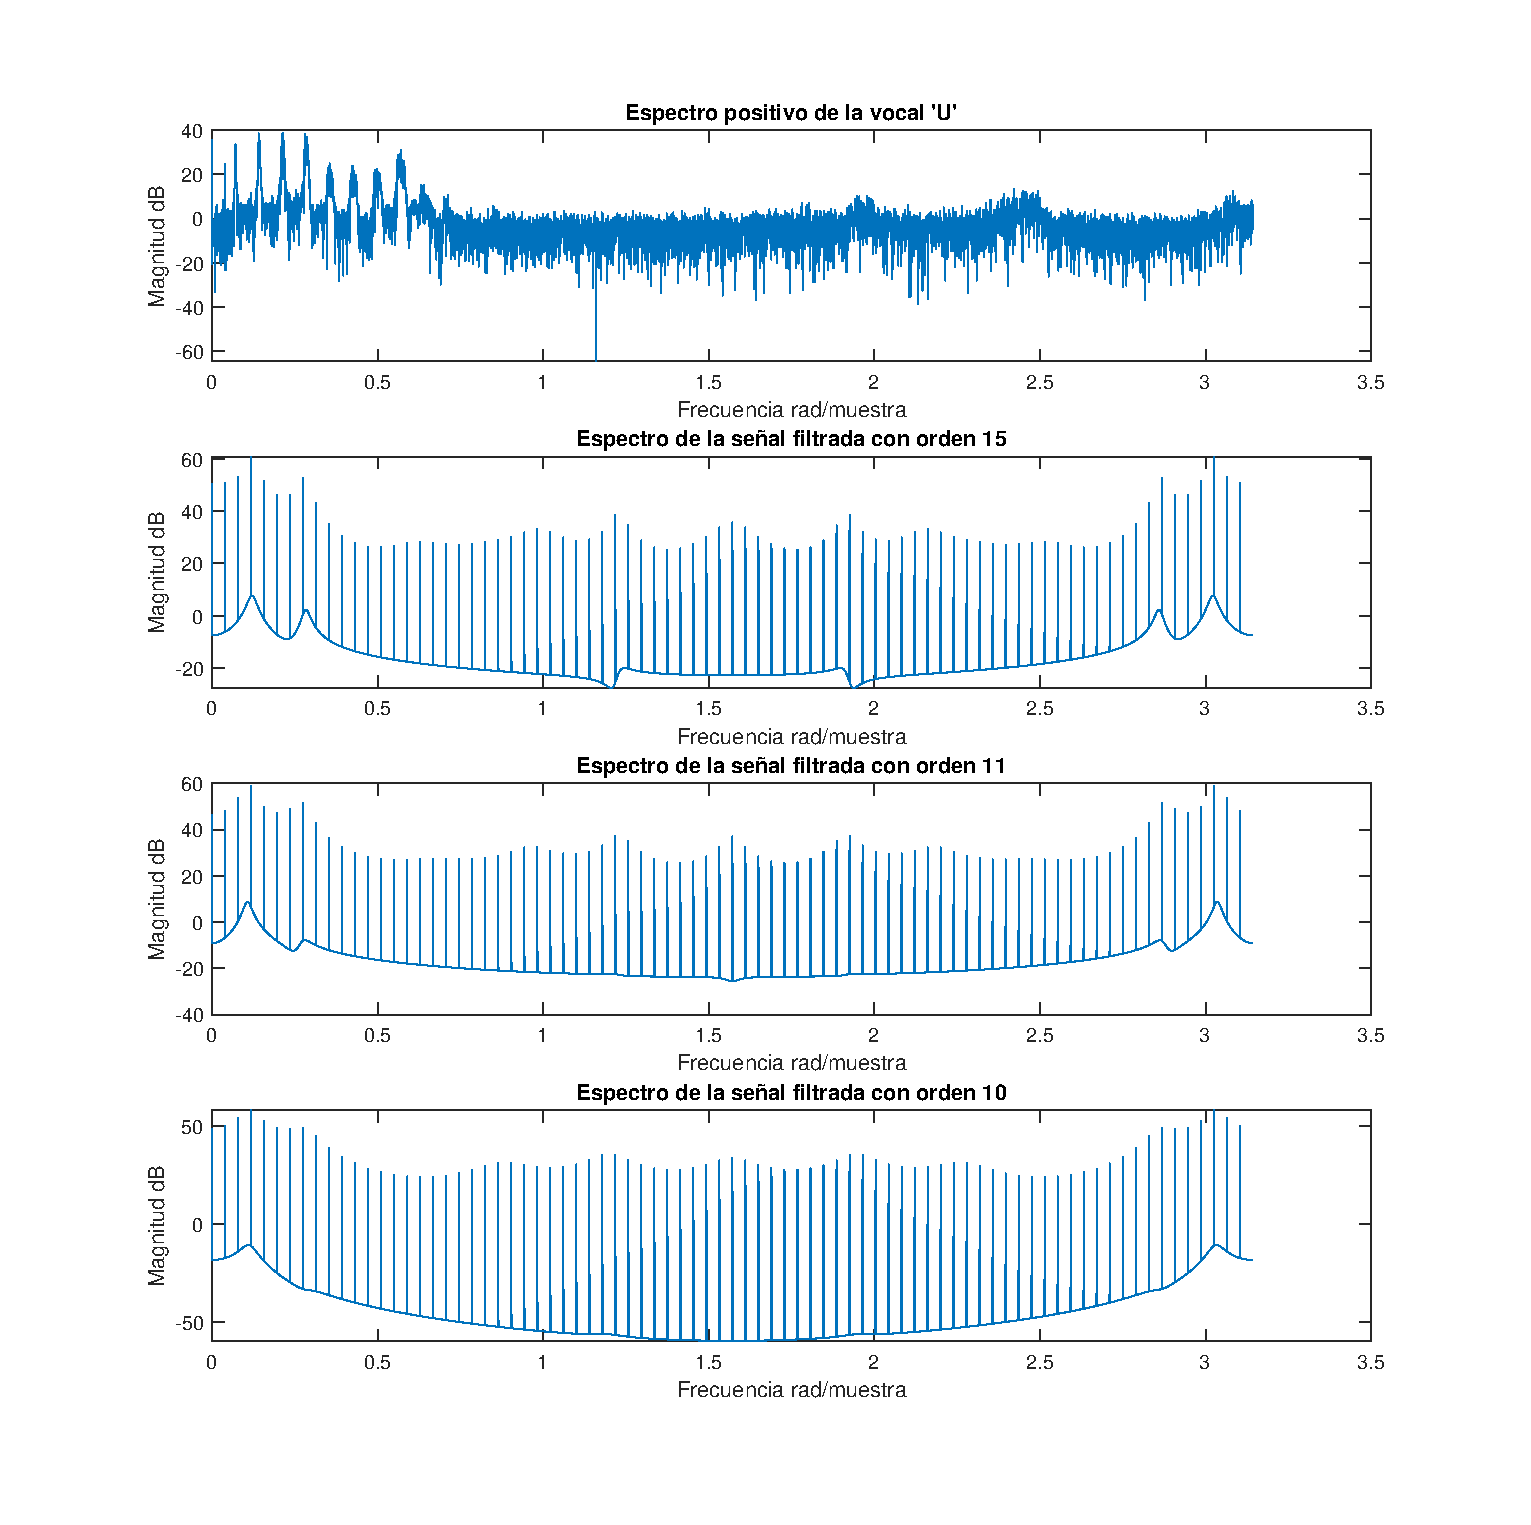
\includegraphics[scale = 0.5]{figures/4_3_filtradoU.eps}
    \caption{Espectro en frecuencia de la señal \textit{vowels\_u} y el resultado de filtrado de orden 15 y 10 }
    \label{AR-15-10}
\end{figure}

\begin{figure}[H]
    \centering
    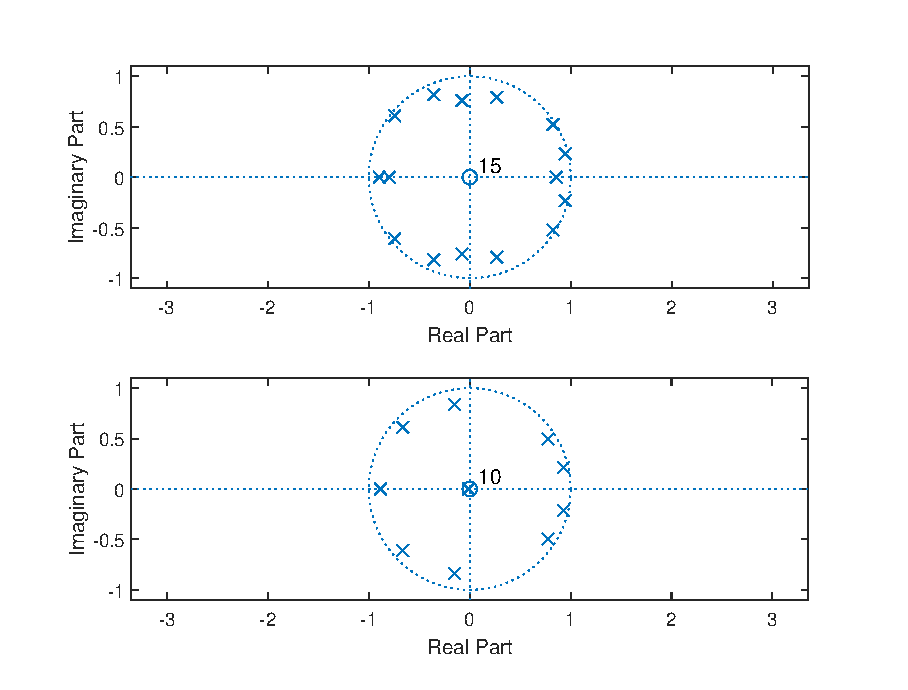
\includegraphics[scale = 0.8]{figures/4_3_zplaneu.eps}
    \caption{Diagramas de polos y ceros para los filtros AR de orden 15 y 10}
    \label{zplane1}
\end{figure}


De la figura \ref{AR-15-10} se puede ver que en el espectro de la vocal \textit{U} se ven 5 formantes, y el orden mínimo que permitía una síntesis de la señal sin diferencias significativas fue 11. Por otro lado en en la figura \ref{frec_A_positive} de la sección 4.1 se encontraron 4 formantes y cuando se sintetizó la señal con un filtro de orden 9 no se notaron diferencias significativas respecto al filtrado de orden 15, con esto se puede concluir que un buen criterio para lograr una buena síntesis de este tipo de señales es encontrando el orden según $2n + 1$, siendo $n$ el número de formantes de la señal a sintetizar.
%%%%%%%%%%%%%%%%%%%%%%%%%%%%%%%%%%%%%%%%%%%%%%%%%%%%%%%%%%%%
\subsection{Filtro AR con filtros \textit{ \textit{Biquad}}}

El procedimiento que hasta ahora se ha  llevado a cabo haciendo uso de filtros AR de distintos ordenes se puede homologar mediante el procesamiento en cascada de la señal con múltiples filtros \textit{ \textit{Biquad}} como los estudiados en experiencias anteriores. Matlab provee de la función  \texttt{tf2sos(b,a)} que recibe como parámetros los coeficientes $a_k$ y $b_k$ de un filtro y entrega la matriz sos, que contiene en sus $n/2$ filas en caso de que n sea par y $n/2 + 1$, donde n corresponde al orden del filtro original. Cada fila contiene los coeficientes del numerador y denominador $A_k$ Y $B_k$ de los filtros \textit{\textit{ \textit{Biquad}}} necesarios para que, de en forma de cascada filtren una señal y obtengan el resultado del filtro original. El comando además entrega el  parámetro \textit{g} correspondiente a la ganancia que poseen los filtros \textit{\textit{ \textit{Biquad}}}  entregados en la matriz.


Se experimenta el uso de la función  antes descrita para un filtro AR de orden 15 obtenido al usar el comando \texttt{lpc} para la señal \textit{vowel\_a}, se obtiene la respuesta en frecuencia de cada filtro  \textit{Biquad} entregado en la matriz permitiendo analizar el aporte individual de cada una de ellas en la respuesta en frecuencia total. Se grafican dichas respuestas en frecuencia  forma superpuesta como se puede ver en la figura \ref{Biquads}.


\begin{figure}[H]
    \centering
    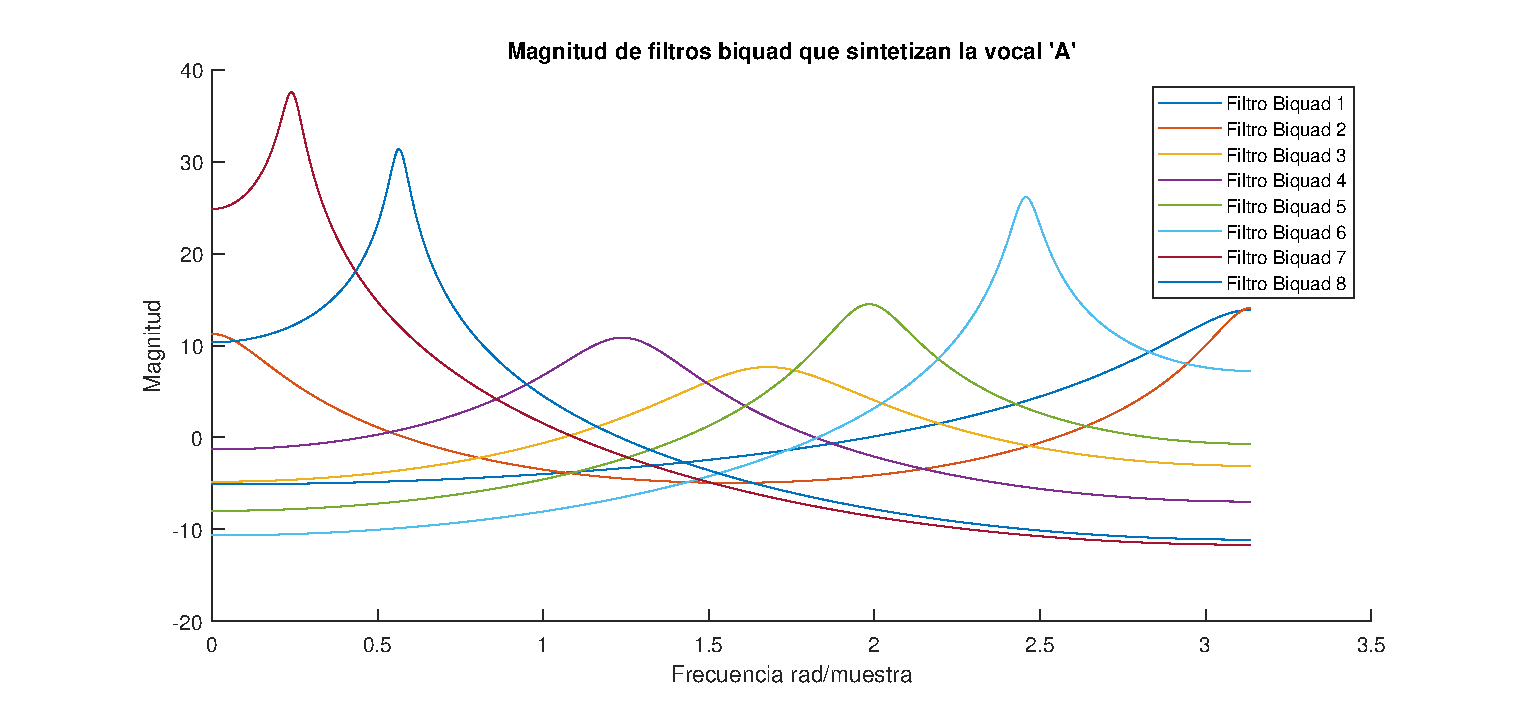
\includegraphics[scale = 0.6]{figures/4_4.eps}
    \caption{Magnitud en $dB$ de la respuesta en frecuencia de los filtros \textit{ \textit{Biquad}} entregados por la función \texttt{tf2sos(b,a)}}
    \label{Biquads}
\end{figure}


Se grafican además de forma superpuesta las magnitudes de las respuestas en frecuencia de los filtros junto al espectro de la señal \textit{vowel\_a} como se muestra en la figura \ref{Biquadss_vocal}

\begin{figure}[H]
    \centering
    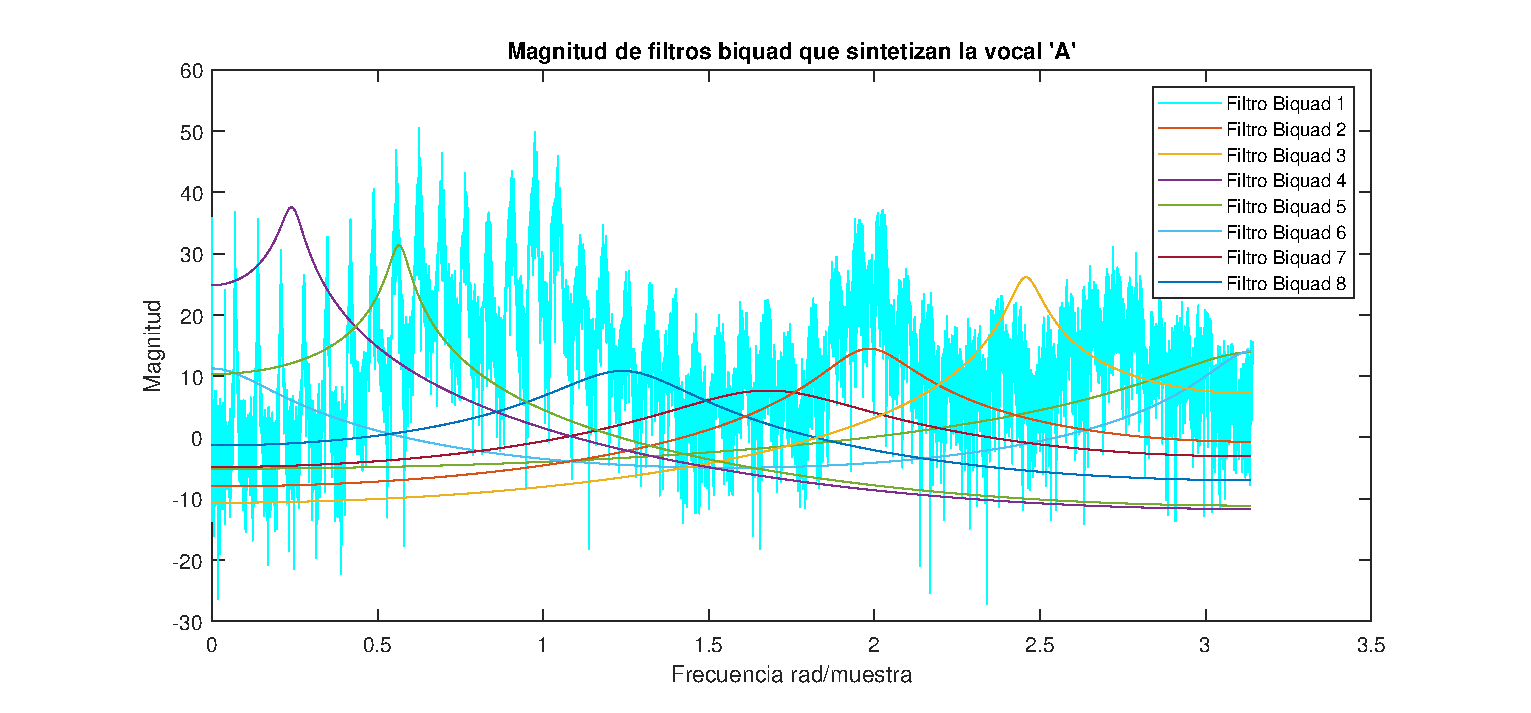
\includegraphics[scale = 0.6]{figures/4_4_vocal.eps}
    \caption{Magnitud en $dB$ de la respuesta en frecuencia de los filtros \textit{ \textit{Biquad}} entregados por la función tf2sos(b,a) junto al espectro de la vocal \textit{A}}
    \label{Biquadss_vocal}
\end{figure}






\clearpage

%V
\section{Observando el residuo de predicción}

Para esta parte se utiliza el script \texttt{p5.m}, el cual se adjunta a la entrega

Para lo que sigue de la sección, se considera $e[n]$ como la señal de entrada a filtro AR. Por lo tanto
$$ X(z) = E(z)\cdot H(z)$$
\subsection{Filtro inverso}
Se puede obtener el filtro inverso al AR como el filtro $H(z)^-1$, el cual corresponde a un filtro FIR. A partir de lo anterior se la respuesta en frecuencia del filtro inverso, la cual se muestra en la figura \ref{fig:p5_1}

\begin{figure}[H]
    \centering
    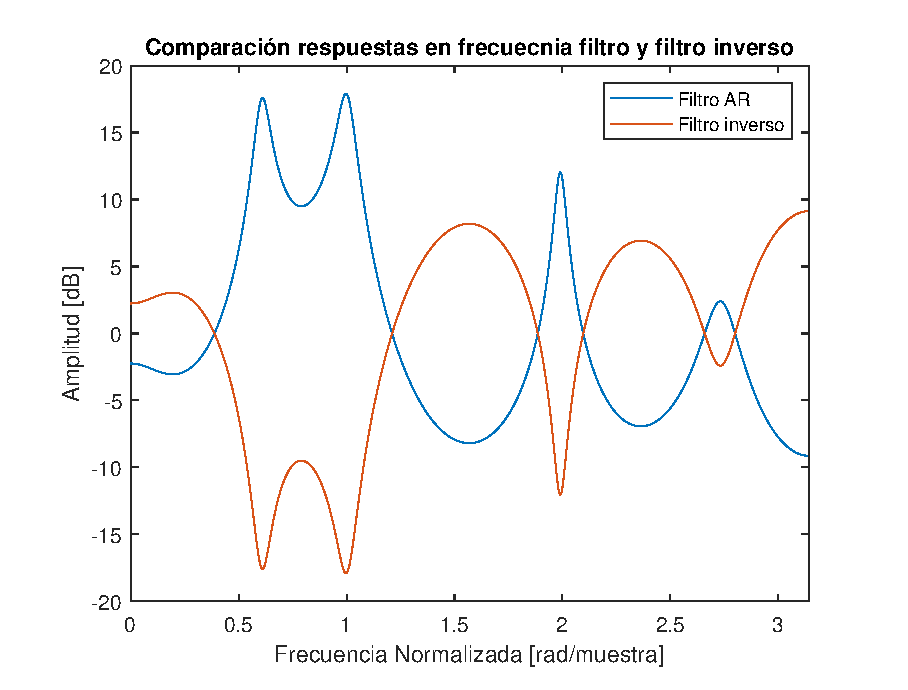
\includegraphics[width = .8\linewidth]{figures/p5_1filtinv.eps}
    \caption{Comparación de respuesta en frecuencia de filtro y filtro inverso.}
    \label{fig:p5_1}
\end{figure}

Como es de esperarse, suma de la respuesta en frecuencia del filtro inverso con el filtro AR es 0.
%%%%%%%%%%%%%%%%%%%%%%%%%%%%%%%%%%%%%%%%%%%%%%%%%%%%%%%%%%%%%%%%%%%%
\subsection{Obtención de la $e[n]$}

Se obtiene $e[n]$ aplicando el filtro inverso a la señal $vowel\_a$. La señal de entrada obtenida se muestra en la figura \ref{fig:p5_2}.

\begin{figure}[H]
    \centering
    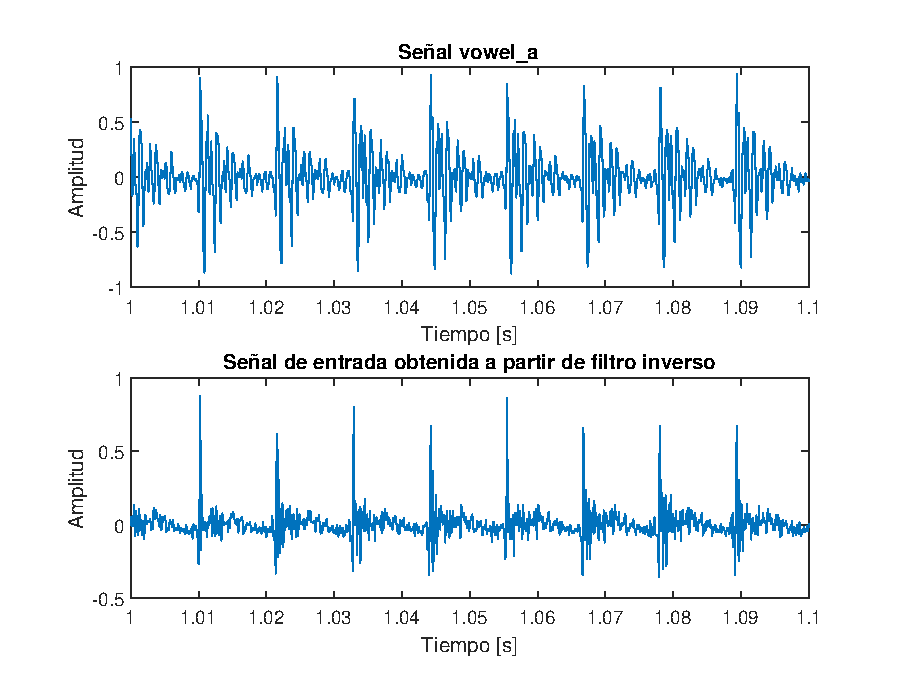
\includegraphics[width = .8\linewidth]{figures/p5_2.eps}
    \caption{Señal $vowel\_a$ y entrada $e[n]$ según filtro inverso.}
    \label{fig:p5_2}
\end{figure}

Con respecto a la forma de la señal $e[n]$ se pueden comentar que:
\begin{itemize}
    \item Modelar la entrada como un tren de impulsos para síntesis no está tan alejado de la entrada ''real'', por lo menos visualmente.
    \item La entrada tiene cierta periodicidad, por lo que se podría modelar como un tren de impulsos convolucionado con otra señal. Lo anterior puede interpretarse como que esta otra señal podría ser parte de la respuesta a impulso que el filtro AR no fue capaz de capturar (respuesta a impulso del tracto vocal). Otra interpretación sería que corresponde a la respuesta impulso de un sistema que no corresponde al del tracto vocal, como podría ser del equipo con el que se grabó o del lugar.
\end{itemize}

\subsection{Espectro en frecuencia de $e[n]$ y $vowel\_a$}

Se grafica el espectro en frecuencia de $e[n]$ y la señal $vowel\_a$, los cuales se muestran en la figura \ref{fig:p5_3}. Con respecto a los gráficos obtenidos se puede comentar que:
\begin{itemize}
    \item La señal $e[n]$ tiene un contenido en frecuencia aproximadamente plano.
    \item La respuesta en frecuencia del filtro AR de a empieza a parecer la envolvente del espectro de $vowel\_a$ debido a la naturaleza plana y ruidosa de $e[n]$. 
\end{itemize}

\begin{figure}[H]
    \centering
    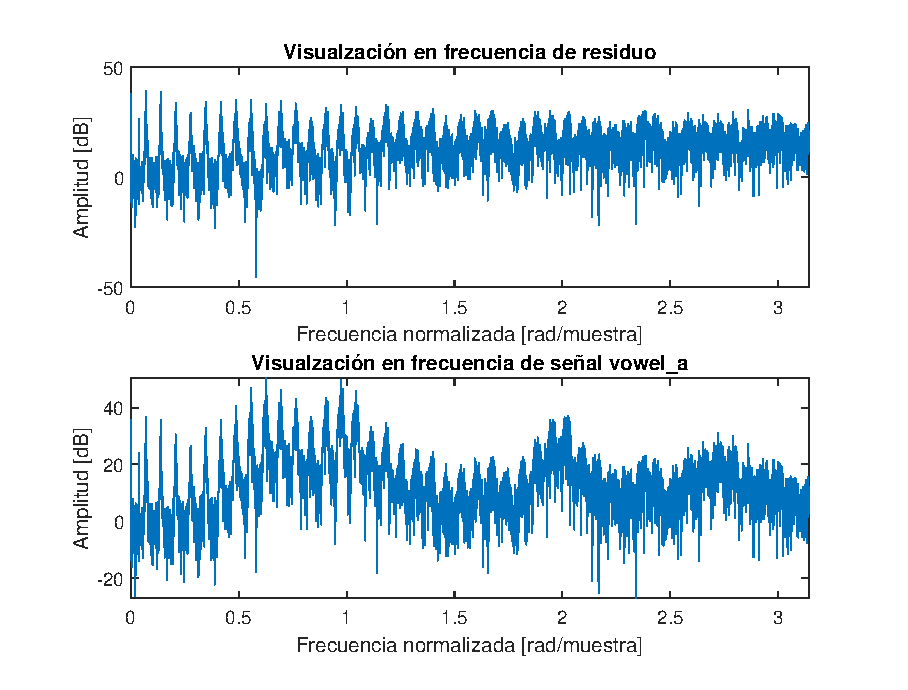
\includegraphics[width = .8\linewidth]{figures/p5_3.eps}
    \caption{Espectro en frecuencia de $e[n]$ y $vowel\_a$}
    \label{fig:p5_3}
\end{figure}

\subsection{Autocorrelación del Residuo y Frecuencia Fundamental}

Se obtiene la autocorrelación del residuo $e[n]$ y de la señal $vowel\_a$. Ambas señales se muestran en los gráficos presentes en la figura \ref{fig:p5_4}.

Para estimar la frecuencia fundamental la autocorrelación de $e[n]$ resulta bastante útil. Un peak en la autocorrelación significa que la señal tiene un gran parecido con respecto a dicho desfase de muestras, por lo que una señal que presente cierta periodicidad debiese tener peaks periódicos en su estimador de autocorrelación.

En el caso de la figura \ref{fig:p5_4}, se aprecian peaks periódicos cada un desfase $D$ aproximado de 90 muestras, por lo que la frecuencia fundamental podría estimarse como:
$$f_0 = \dfrac{1}{D\cdot T_s} =  \dfrac{1}{90\cdot (1/8000)} \approx 88.9~Hz$$

\begin{figure}[H]
    \centering
    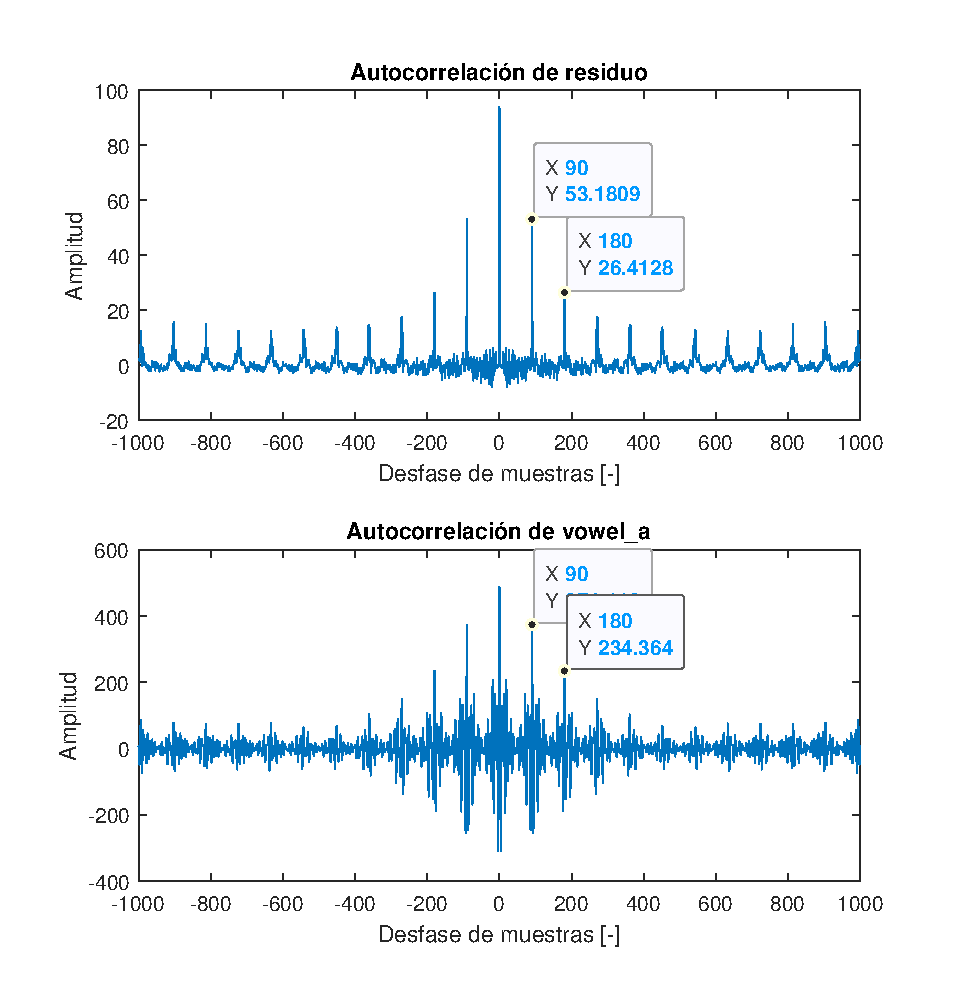
\includegraphics[width = .8\linewidth]{figures/p5_4.eps}
    \caption{Autocorrelación de $e[n]$ y $vowel\_a$}
    \label{fig:p5_4}
\end{figure}

Este método de estimación depende de que la señal este poco correlacionada en el entorno del desfase $D$ respectivo a la fundamental. De no ser así complicaría encontrar el peak, lo cual se puede apreciar levemente en la autocorrelación del la señal $vowel\_a$, ya que si bien los peaks ''importantes'' para estimar la frecuencia fundamental aún son distinguibles, un filtro de respuesta a impulso más ancha haría la tarea más complicada.

\clearpage

\end{document}

